\documentclass[a4paper]{report}
\usepackage[utf8]{inputenc}
\usepackage[T1]{fontenc}
\usepackage{RJournal}
\usepackage{amsmath,amssymb,array}
\usepackage{booktabs}


% tightlist command for lists without linebreak
\providecommand{\tightlist}{%
  \setlength{\itemsep}{0pt}\setlength{\parskip}{0pt}}

\usepackage{longtable}

% Always define CSL refs as bib entries are contained in separate doc
% Pandoc citation processing
\newlength{\cslhangindent}
\setlength{\cslhangindent}{1.5em}
\newlength{\csllabelwidth}
\setlength{\csllabelwidth}{3em}
\newlength{\cslentryspacingunit} % times entry-spacing
\setlength{\cslentryspacingunit}{\parskip}
% for Pandoc 2.8 to 2.10.1
\newenvironment{cslreferences}%
  {}%
  {\par}
% For Pandoc 2.11+
\newenvironment{CSLReferences}[2] % #1 hanging-ident, #2 entry spacing
 {% don't indent paragraphs
  \setlength{\parindent}{0pt}
  % turn on hanging indent if param 1 is 1
  \ifodd #1
  \let\oldpar\par
  \def\par{\hangindent=\cslhangindent\oldpar}
  \fi
  % set entry spacing
  \setlength{\parskip}{#2\cslentryspacingunit}
 }%
 {}
\usepackage{calc}
\newcommand{\CSLBlock}[1]{#1\hfill\break}
\newcommand{\CSLLeftMargin}[1]{\parbox[t]{\csllabelwidth}{#1}}
\newcommand{\CSLRightInline}[1]{\parbox[t]{\linewidth - \csllabelwidth}{#1}\break}
\newcommand{\CSLIndent}[1]{\hspace{\cslhangindent}#1}


\usepackage[labelformat=simple]{subcaption}
\renewcommand\thesubfigure{(\alph{subfigure})}
\usepackage{tikz,enumitem}
\usetikzlibrary{positioning, arrows.meta, shapes.geometric}
\tikzset{%
  semithick,
  >={Stealth[width=2mm, length=2.75mm]},
  obs/.style = {name = #1, circle, draw, inner sep = 5pt, label = center:\(\scriptstyle#1\)},
  fixed/.style = {name = #1, regular polygon, regular polygon sides = 4, draw, inner sep = 3pt, label = center:\(#1\)},
  lat/.style 2 args = {name = #1, circle, draw, dashed, inner sep = 5pt, label = center:\(\scriptstyle#2\)},
}
%\newtheorem{lemma}{Lemma}
\newcommand\independent{\protect\mathpalette{\protect\independenT}{\perp}}
\def\independenT#1#2{\mathrel{\rlap{\(#1#2\)}\mkern2mu{#1#2}}}
\newcommand{\+}[1]{\ensuremath{\mathbf{#1}}}
\newcommand{\doo}{\textrm{do}}


\begin{document}


%% do not edit, for illustration only
\sectionhead{Contributed research article}
\volume{15}
\volnumber{3}
\year{2023}
\month{September}
\setcounter{page}{138}

\begin{article}
  % !TeX root = RJwrapper.tex
\title{bayesassurance: An R Package for Calculating Sample Size and Bayesian Assurance}


\author{by Jane Pan and Sudipto Banerjee}

\maketitle

\abstract{%
In this paper, we present bayesassurance, an {R} package designed for computing Bayesian assurance criteria which can be used to determine sample size in Bayesian inference setting. The functions included in the {R} package offer a two-stage framework using design priors to specify the population from which the data will be collected and analysis priors to fit a Bayesian model. We also demonstrate that frequentist sample size calculations are exactly reproduced as special cases of evaluating Bayesian assurance functions using appropriately specified priors.
}

\section{Introduction}\label{introduction}

Power is an important feature of statistical tests that refers to the probability of correctly identifying the occurrence of an event given the event is actually present. %In the classical setting, identifying an appropriate sample size to achieve a desired statistical power offers valuable insight when making decisions. 
Specifically, in the frequentist setting, the power of a test describes the probability that the test will correctly reject the null hypothesis, $H_0$, given that the alternative hypothesis, $H_1$,  is true. Conversely, $\beta = 1 - \text{power}$ represents the probability that a test will fail to identify a true effect. For any given test, power is a function of the underlying effect size, the significance level, $\alpha$, and the sample size, $n$ . While the underlying effect size is rarely under the experimenter's control, the significance level and the sample size are. Hence, it is important to conduct power analysis to determine appropriate assignments of $\alpha$ and $n$  for an experiment to have a good chance of detecting an effect if one exists. 
%Power and sample size analysis constitutes an essential component of statistical designs for scientific experiments. 
Power curves serve as a useful tool in quantifying the degree of assurance held towards meeting a study's analysis objective across a range of sample sizes. Formulating sample size determination as a decision problem so that power is an increasing function of sample size, offers the investigator a visual aid in helping deduce the minimum sample size needed to achieve a desired power. 

The analogue of power in the Bayesian setting is \emph{assurance}, which is based upon the probability of meeting a desired analysis objective. As an example, our analysis objective could be to ascertain if the difference between two population quantities, $\theta_1$ and $\theta_2$, exceeds a certain threshold $\theta_0$, i.e., $\theta_1 - \theta_2 > \theta_0$. We decide that our analysis objective is met if the posterior probability of the above event given data we have observed exceeds $\omega$, i.e., $P(\theta_1 - \theta_2 > \theta_0 \mid y) > \omega$ with $y$ being the realized data. Assurance is defined as the probability of the analysis objective being met under an assumed distribution of the data, i.e., $\delta = P_{y}\left\{y: P\left(\theta > \theta_0 \mid {y}\right) > \omega \right\}$, where ${y}$ denotes the observed data. Several publications adopt a similar approach, where they determine sample size based upon some criteria of analysis or model performance \citep{rahme, wang, ohagan}. Other proposed solutions of the sample size problem introduce frameworks that prioritize conditions specific to the problem at hand, e.g. the use of Bayesian average errors to simultaneously control for Type I and Type II errors \citep{reyes}, the use of posterior credible interval lengths to evaluate
sample size estimates \citep{joseph}, and the use of survival regression models to target
Bayesian meta-experimental designs \citep{reyes}.

\begin{table}[t!]
\centering
\begin{tabular}{lllp{6.2cm}}
\hline
Function  & Type & & Description \\ \hline
\fct{pwr\_freq} & closed-form solution & &
Computes the frequentist power
of the specified hypothesis test (either
one or two-sided $z$-tests).  \\
\fct{assurance\_nd\_na} & closed-form solution & & Computes 
the exact Bayesian assurance of 
attaining a specified analysis objective.\\
\fct{bayes\_sim} & simulation & & Approximates the Bayesian assurance of attaining a specified
condition for a balanced study design through 
Monte Carlo sampling.\\
\fct{bayes\_sim\_unbalanced} & simulation & & 
Approximates the Bayesian assurance of attaining 
a specified condition for an unbalanced study 
design through Monte Carlo sampling.\\
\fct{bayes\_sim\_unknownvar} & simulation & & 
Similar to \fct{bayes\_sim} but approximates the assurance
assuming unknown variance.\\
%Approximates the Bayesian assurance of attaining 
%a specified condition through Monte Carlo 
%sampling with the added assumption that 
%the variance is unknown.\\
\fct{bayes\_adcock} & simulation & & 
%Approximates the assurance of observing that the absolute difference between the true underlying population parameter and the sample estimate falls within a margin of error no greater than a fixed precision level, $d$.
Approximates the probability (assurance)
that the absolute difference between the true population
parameter and the sample estimate falls within a margin 
of error no greater than a pre-specified precision level, $d$
\citep{cj}. 
\\
\fct{bayes\_sim\_betabin} & simulation & &
Approximates the probability (assurance) that
there exists a difference between two independent proportions
\citep{pham}.\\
\fct{bayes\_goal\_func} & simulation & &
Approximates the rate of correct classification 
using a utility-based approach within a linear hypothesis
testing setting \citep{inoue}.\\
\fct{pwr\_curve} & visual tool & & Constructs a plot
with the power and assurance curves overlayed on top
of each other for comparison. \\
\fct{gen\_Xn} & design tool & &
Constructs design matrix using given sample size(s).
Used for power and sample size analysis in the Bayesian setting. \\
\fct{gen\_Xn\_longitudinal} & design tool & &
Constructs design matrix using inputs that correspond
to a balanced longitudinal study design.\\
 \\ \hline
\end{tabular}
\caption{Overview of the
functions available for use within the package.}\label{tab:overview}
\end{table}

There are several \proglang{R} packages for Bayesian sample size determination using specified analytic criteria. The \pkg{SampleSizeMeans} package %produced by Lawrence Joseph and Patrick Belisle 
contains a series of functions used for determining appropriate sample sizes based on various Bayesian criteria for estimating means or differences between means of normal variables \citep{samplesizemeans}. Criteria considered include the Average Length Criterion,  the Average Coverage Criterion, and the  Modified Worst Outcome Criterion  \citep{joseph1995, joseph1997}. A supplementary package, \pkg{SampleSizeProportions}, addresses study designs for estimation of binomial proportions using the same set of criteria \citep{samplesizeprop}. 
%Additionally, there is also an \pkg{assurance} R package
%(cite Paul Metcalfe) that presents tools for 
%computing assurance using a standard posterior 
%sampling approach, specifically in the context of 
%binomial and negative binomial regression models,
%Gaussian endpoints, and multiple correlated endpoints.   
Our package, \pkg{bayesassurance} calculates Bayesian assurance and sample sizes for analysis objectives using normal and binomial models. We devise a two stage framework using possibly different sets of prior distributions in the design and analysis stages. The prior in the design stage represents a model that generates the data. The prior in the analysis stage represents the analyst's beliefs about the data. These two prior distributions are possibly different because the analyst does not usually have enough prior information on the processes generating the data. We primarily demonstrate sample size determination using conjugate Bayesian linear regression models as a prototype for this article, although the \proglang{R} package offers functions for calculating Bayesian assurance for binary or binomial models as well. In the current article, we focus on the flexibility of Bayesian linear regression models and demonstrate determination of unequal sample sizes for two samples and longitudinal study designs. 

The \pkg{bayesassurance} package is available on CRAN \citep{bayesassurance} and contains a collection of functions that can be divided into three categories based on design and usage. These include closed-form solutions, simulation-based solutions, and visualization and/or design purposes. All available functions are presented in Table~\ref{tab:overview}.
%The manuscript is organized as follows. Section~\ref{sec:closedformassurance} 
%All of the simulation-based functions follow a similar format and require a similar set of specifications. Hence, for brevity, we do not go over every function in detail. 
Fully worked-out examples and tutorials can be found on our Github page at  \href{https://github.com/jpan928/bayesassurance_rpackage}{https://github.com/jpan928/bayesassurance\_rpackage}. This article describes the basic underlying framework leading to analytically tractable expressions for Bayesian assurance. We will also illustrate the relationship between Bayesian and frequentist sample size determination.
%Sections~\ref{sec:simform} and~\ref{sec:othermethods}
In addition, we briefly explore simulation-based assurance methods, outlining the statistical distribution theory associated with each method, followed by examples worked out in \proglang{R} that users will be able to replicate. 
%Section~\ref{sec: goalfunc} discusses a related topic similar to the assurance that determines sample size in relation to the rate of correct classification. Here we discuss how a Bayesian goal function is formulated and applied in the context of sample size determination. 
Finally, we offer some useful graphical features and design matrix generators offered by the package. In the following sections, we provide a detailed overview for each of the available functions grouped  by category followed with worked out examples in \proglang{R}. 




\section{Closed-form Solution of Assurance}\label{sec:closedformassurance}
Bayesian assurance evaluates the tenability of attaining a specified outcome through the implementation of prior and posterior distributions.  The \fct{assurance\_nd\_na} function computes the exact assurance using a closed-form solution. Classical frequentist (Neyman-Pearson) inference proceeds as follows. Prior to an experiment, the analyst determines the sample size, as well as significance level ($\alpha$), which defines the maximum frequency of false positives (type I errors) they are willing to tolerate, if the null hypothesis is true. Then, once the data has been collected, a statistical test is conducted which yields the p-value or the probability of seeing the observed data under the null hypothesis. If the p-value is lower than $\alpha$, the null hypothesis is rejected. In contrast, in Bayesian inference refrains from ``rejecting'' or ``failing to reject the null hypothesis''. Instead, we look at the tenability of a hypothesis based upon realized data. As an example, suppose we seek to evaluate the tenability of $H : \theta > \theta_0$ given data from a Gaussian population with mean $\theta_0$ and known variance $\sigma^2$. We assign two sets of priors for $\theta$, one at the $\textit{design stage}$ and the other at the  $\textit{analysis stage}$. These two stages are the  primary components that make up the skeleton of our generalized solution in the Bayesian setting and will be revisited in later sections. The analysis objective specifies the condition that needs to be satisfied. It defines a positive outcome, which serves as an overarching criteria that characterizes the study. 
%The analysis objective
%defines a positive outcome that serves as an 
%overarching criteria characterizing the study. 
%In this setting, 
{O}ur analysis objective is to ascertain if
$P(\theta > \theta_0 \mid \bar{y}) > 1-\alpha$, where $\bar{y}$ is the data average and 
$\alpha$ is a specified threshold.  Assuming the prior $\theta \sim N\left(\mu, \frac{\sigma^2}{n_a}\right)$, the posterior distribution of $\theta$ is
\begin{equation}\label{eq: simple_posterior}
N\left(\theta {\, \left | \, \mu, \frac{\sigma^2}{n_a} \right.}\right) \times N\left(\bar{y} {\, \left |\, \theta, \frac{\sigma^2}{n} \right.}\right)
\propto N\left(\theta {\, \left |\, \frac{n_a}{n + n_a}\mu + \frac{n}{n + n_a}\bar{y}, \frac{\sigma^2}{n + n_a}\right.}\right)\;,
\end{equation}
where $n$ denotes the sample size of the data, $\bar{y}$ denotes the mean of the data, and $n_a$ is specified by the data analyst to quantify the prior degree of belief on $\theta$.

The design objective is to find the sample size needed to ensure that the analysis objective is met $100\delta\%$ of the time, where $\delta$ denotes the assurance. At the design stage, we specify a model for the underlying population from which the data is generated. Our belief about this population is quantified using a \emph{design prior} \citep[we borrow this terminology from ][]{ohagan}, say $\theta \sim N\left(\mu, \frac{\sigma^2}{n_d}\right)$, where $n_d$ is specified by the user to quantify the degree of belief (or amount of confidence) on the population parameters. %Then given the likelihood $\bar{y} \sim N\left(\theta, \frac{\sigma^2}{n}\right)$ 
Bayesian assurance is given by
\begin{equation}\label{eq:assurance_general}
\delta = P_{\bar{y}}\left\{\bar{y}: P(\theta > \theta_0 \mid \bar{y}) > 1 - \alpha\right\}\;,
\end{equation}
where $P_{\bar{y}}(\cdot)$ denotes the marginal distribution of $\bar{y}$ obtained from the design priors 
\[
\int{N\left(\theta {\,\left|\,\mu, \frac{\sigma^2}{n_d}\right.}\right) \times N\left(\bar{y} {\,\left |\, \theta, \frac{\sigma^2}{n} \right.}\right) d\theta} 
= N\left(\bar{y} {\,\left |\,\mu, \left(\frac{1}{n} + \frac{1}{n_d}\right) \sigma^2 \right.}\right)\;.
\]
Applying this to (\ref{eq:assurance_general}) we obtain
\begin{equation} \label{eq:assurance}
\delta(\Delta, n) = \Phi\left(\sqrt{\frac{nn_d}{n+n_d}}
\left[\frac{n+n_a}{n}\frac{\Delta}{\sigma} + Z_{\alpha}\frac{n+n_a}{n}\right]\right)\;,
\end{equation}
where $\Phi(\cdot)$ is the standard normal CDF with $Z_{\alpha}$ being its $\alpha$-th quantile and $\Delta = \mu - \theta_0$. 

We remark that the above expression assumes that $\sigma^2$ is known. This is a customary assumption made about the population in sample size calculations and is usually based upon pilot studies or historic data. Nevertheless, in theory we can relax this assumption and assign a prior distribution to $\sigma^2$. Conjugate priors include the inverse-Gamma family of distributions and analogous formulas to (\ref{eq:assurance}) may be derived in terms of distribution functions of the (non-central) t-distribution. Nevertheless, we do not pursue this development here but discuss the case of unknown $\sigma^2$ later in the linear regression setting. We now describe the function to compute (\ref{eq:assurance}).
Table~\ref{tab:assurance_nd_na} lists the set of parameters used in \fct{assurance\_nd\_na}, with \code{alpha} taking a default value of 0.05. 

\begin{table}[t!]
    \centering
    \begin{tabular}{|p{3cm}||p{8.5cm}|}
    \hline
    \multicolumn{2}{|l|}{\fct{assurance\_nd\_na:} \textbf{Parameters}}\\
    \hline
    \hline
    Variable  & Description \\ 
    \hline
    \hline
         n & sample size (either scalar or vector)\\
         \hline
         \code{n\_a} & precision parameter within the analysis
         stage that quantifies the degree of belief carried towards 
         parameter $\theta$\\
         \hline
         \code{n\_d}& precision parameter within the design stage
         that quantifies the degree of belief of the population from 
         which we are generating samples from\\
         \hline
         \code{theta\_0}& initial parameter value provided by the client\\
         \hline
         \code{theta\_1}& prior mean of $\theta$ assigned in the
         analysis and design stage\\
         \hline
         \code{sigsq}& known variance\\
         \hline
         \code{alt}& specifies alternative test case, 
         where \code{alt = "greater"} tests if 
         $\theta_1 > \theta_0$,\code{ alt = "less"} tests if 
         $\theta_1 < \theta_0$, and \code{alt = "two.sided"}
         performs a two-sided test for 
         $\theta_1 \neq \theta_0$.  By default, 
         \code{alt = "greater"}\\
         \hline
         \code{alpha}& significance level\\
         \hline
    \end{tabular}
    \caption{Parameter specifications needed to run \fct{assurance\_nd\_na}.}
    \label{tab:assurance_nd_na}
\end{table}

 
The following code loads the  \pkg{bayesassurance} package and assigns arbitrary parameters to \fct{assurance\_nd\_na} prior to executing the function. 
\begin{Schunk}
\begin{Sin}

R> library(bayesassurance)

R> n <- seq(100, 250, 10)
R> n_a <- 10
R> n_d <- 10
R> theta_0 <- 0.15
R> theta_1 <- 0.25
R> sigsq <- 0.30

R> out <- assurance_nd_na(n = n, n_a = n_a,  n_d = n_d, 
	theta_0 = theta_0, theta_1 = theta_1, sigsq = sigsq,  
	alt = "greater", alpha = 0.05)

R> head(out$assurance_table)
R> out$assurance_plot

\end{Sin}
\begin{Sout}
     n Assurance
1  100 0.5228078
2  110 0.5324414
3  120 0.5408288
4  130 0.5482139
5  140 0.5547789
6  150 0.5606632
\end{Sout}
\end{Schunk}

\begin{figure}[t!]
\centering
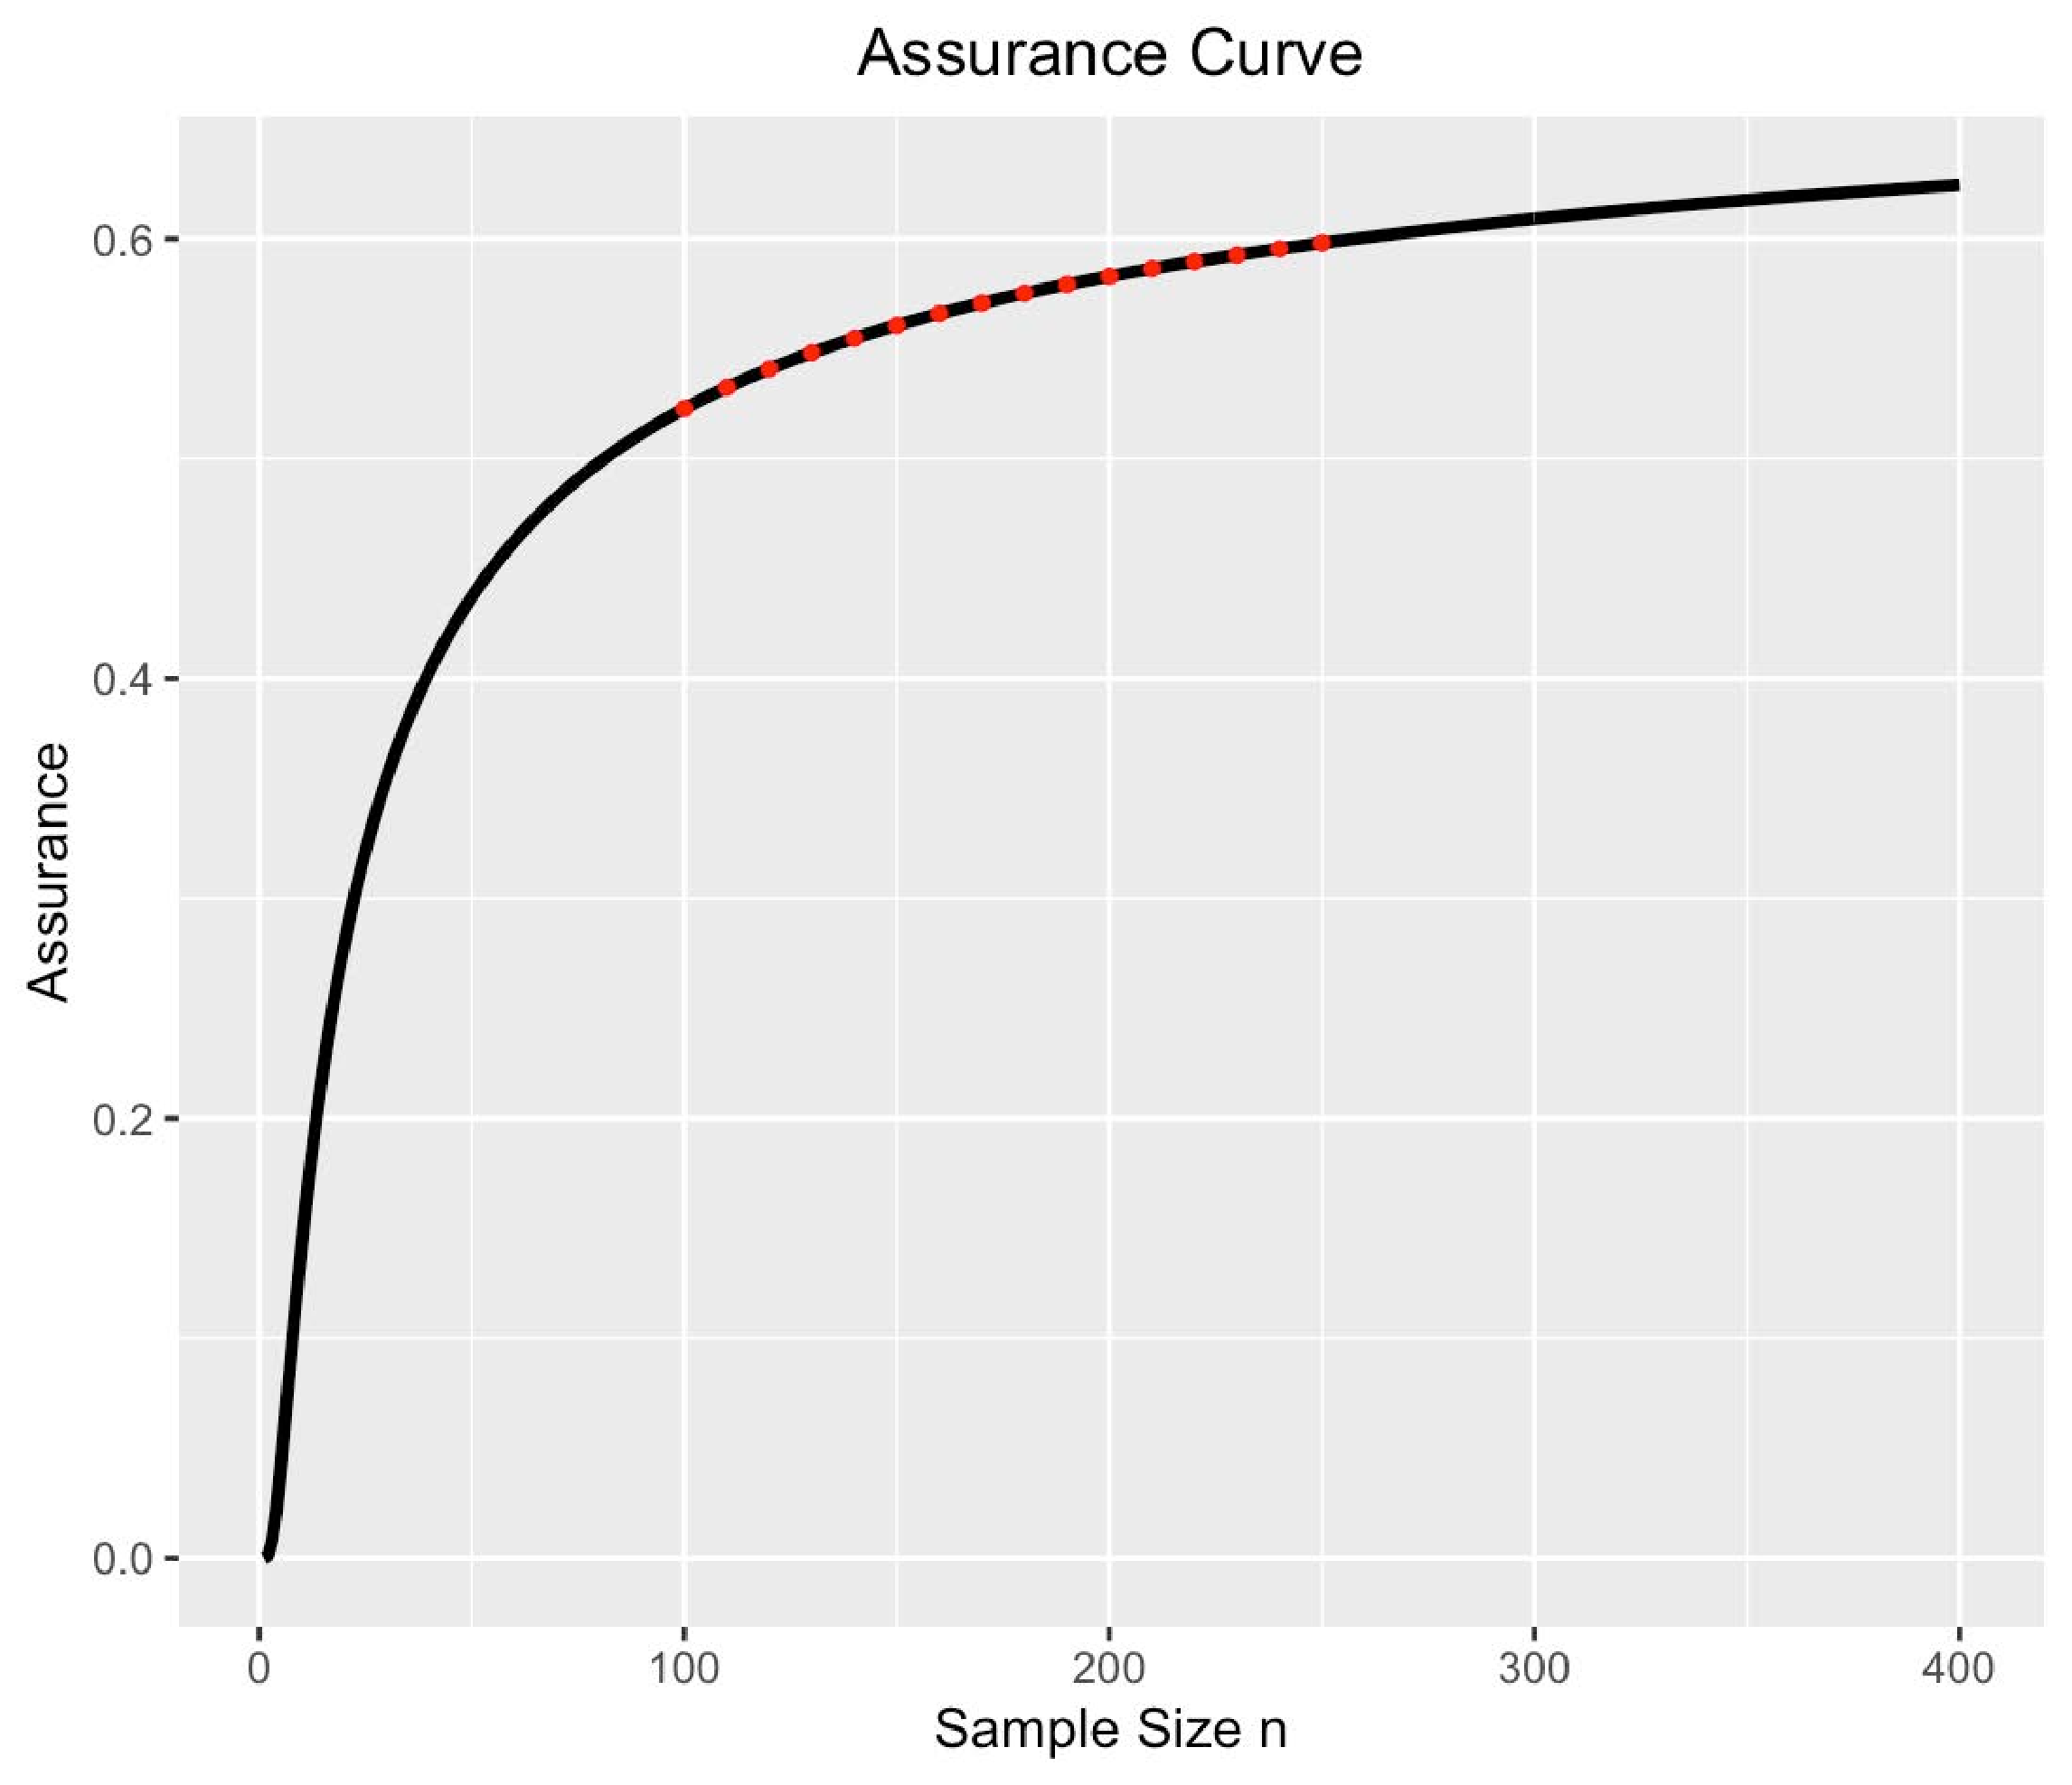
\includegraphics[width = 8 cm]{assur_plot_ex1.pdf}
\caption{\label{fig:assur_plot} Resulting assurance plot
with specific points passed in marked in red.}
\end{figure}

Running this block of code will return a table of assurance values  and a graphical display of the assurance curve, shown in Figure~\ref{fig:assur_plot}. The first six rows of the table are reported in the outputs. 

We make a few remarks pertaining to the functions in \pkg{bayesassurance}.  First, we are passing a single value of sample size or a vector of sample sizes for \code{n}. We save the results as a variable \code{out}. %The list of objects returned by the function depends on whether \code{n} is a scalar or a vector.  
\code{n} can be either a scalar or vector. If \code{n} is a scalar, this tells the function that we only want to determine the assurance for one particular sample size. When this is the case, 
\code{out} will return a single assurance value with no plot. Alternatively, if a vector of sample sizes is passed in as \code{n}, as is the case of the example above, assurance is computed for a list of sample sizes, and the function will produce both a table and an assurance curve showing the results. As long as \code{n} is of length two or greater, \code{assurance\_nd\_na} will plot the assurance curve with red points denoting user-specified assurance values and black points denoting all other points outside those specified points. 
%along with a black curve that connects the points in order of appearance on the $x$-axis using the \fct{geom\_line} function in \pkg{ggplot2}~\cite{ggplot2}. 
%will create a graphical display of the assurance values for an array of sample sizes surrounding those values of \code{n} that were passed in, with specific points of interest labeled in red. 
Figure~\ref{fig:assur_plot} presents the assurance curve resulting from the example. The graph is created using \pkg{ggplot2}~\cite{ggplot2} which is imported into \pkg{bayesassurance}. 
Simply typing \code{out\$assurance\_table} and
\code{out\$assurance\_plot} will display the table and plot respectively in this particular set of examples.

\subsection{Special case: convergence with the frequentist setting}
Depending on how we define the parameters in 
\fct{assurance\_nd\_na}, we can demonstrate a relationship between the Bayesian and classical power analysis. In particular, the classical, or frequentist, power function is a special case of Bayesian solution when letting $n_d \rightarrow \infty$ and $n_a = 0$ in \eqref{eq:assurance}. Therefore, assigning a weak analysis prior and a strong design prior yields
\begin{equation}
\label{eq:assurance_weakprior}
\Phi\Big(\sqrt{n}\frac{\Delta}{\sigma} + Z_\alpha\Big),
\end{equation}
which is equivalent to the frequentist power expression that takes the form
\begin{equation}
\nonumber
1-\beta = P\Big(\bar{y} > \theta_0 +
 \frac{\sigma}{\sqrt{n}}Z_{1-\alpha}\Big) = 
\Phi\Big(\sqrt{n}\frac{\Delta}{\sigma} + Z_\alpha\Big).
\end{equation}
%where $\Phi$ denotes the cumulative distribution function
%of the standard normal and $\Delta = \theta_1 - \theta_0$.
The following code chunk demonstrates this special case 
in \proglang{R} using the \fct{assurance\_nd\_na} function: 

\begin{Schunk}
\begin{Sin}

R> library(bayesassurance)

R> n <- seq(10, 250, 5)
R> n_a <- 1e-8
R> n_d <- 1e+8
R> theta_0 <- 0.15
R> theta_1 <- 0.25
R> sigsq <- 0.104

R> out <- assurance_nd_na(n = n, n_a = n_a,  n_d = n_d, 
        theta_0 = theta_0, theta_1 = theta_1, sigsq = sigsq, 
        alt = "greater", alpha = 0.05)

R> head(out$assurance_table)
R> out$assurance_plot

\end{Sin}
\begin{Sout}
     n Assurance
1   10 0.2532578
2   15 0.3285602
3   20 0.3981637
4   25 0.4623880
5   30 0.5213579
6   35 0.5752063
\end{Sout}
\end{Schunk}


The \pkg{bayesassurance} package includes a \fct{pwr\_freq} function that determines  the statistical power of testing the difference between two means given a set of fixed parameter values that yield a closed-form solution of power and sample size. Continuing with the one-sided
case, the solution is
\begin{equation}
\label{eq:power_func}
1-\beta = P\left(\bar{y} > \theta_0 +
 \frac{\sigma}{\sqrt{n}}Z_{1-\alpha}\right) = 
\Phi\left(\sqrt{n}\frac{\Delta}{\sigma} + Z_\alpha\right),
\end{equation}
where $\Delta = \theta_1 - \theta_0$ is the critical difference and $\Phi$ denotes the cumulative distribution function of the standard
normal. Note this formula is equivalent to the 
special case of the assurance definition expressed in Equation~\eqref{eq:assurance_weakprior}.
Table~\ref{tab:pwr_freq} includes the set of parameters needed to run this function. 

\begin{table}[t!]
    \centering
    \begin{tabular}{|p{3cm}||p{8.5cm}|}
    \hline
    \multicolumn{2}{|l|}{\fct{pwr\_freq:} \textbf{Parameters}}\\
    \hline
    \hline
    Variable  & Description \\ 
    \hline
    \hline
         \code{n} & sample size (either scalar or vector)\\
         \hline
         \code{theta\_0} & value specified in the null 
         hypothesis; to be provided by the user \\
         \hline
         \code{theta\_1} & alternative value to test against the
         null value; this is the assumed effect size in the population \\
         %serves as a threshold in determining whether the null is to be rejected or not\\
         \hline
         \code{alt} & specifies alternative test case, 
         where \code{alt = "greater"} tests if 
         $\theta_1 > \theta_0$,\code{ alt = "less"} tests if 
         $\theta_1 < \theta_0$, and \code{alt = "two.sided"}
         performs a two-sided test for 
         $\theta_1 \neq \theta_0$.  By default, 
         \code{alt = "greater"} \\
         \hline
         \code{sigsq} & known variance \\
         \hline
         \code{alpha}& significance level\\
         \hline
    \end{tabular}
    \caption{Parameter specifications needed to run \fct{pwr\_freq}.}
    \label{tab:pwr_freq}
\end{table}


%\section{Models and software} \label{sec:models}
As a simple example, consider the following code segment
that directly runs \fct{pwr\_freq} through specifying
the above parameters and loading in \pkg{bayesassurance}: 
\begin{Schunk}
\begin{Sin}

R> library(bayesassurance)
R> pwr_freq(n = 20, theta_0 = 0.15, theta_1 = 0.35, sigsq = 0.30, 
		alt = "greater", alpha = 0.05)

\end{Sin}
\end{Schunk}
\begin{Sout}
"Power: 0.495"
\end{Sout}
Running this returns the associated power printed
as a statement rather than a table as we are only passing in one 
sample size, \code{n = 20}, to undergo evaluation. Now consider the next 
code example.
\begin{Schunk}
\begin{Sin}

R> library(bayesassurance)
R> n <- seq(10, 250, 5)
R> out <- pwr_freq(n = n, theta_0 = 0.15, theta_1 = 0.25, sigsq = 0.104, 
        alt = "greater", alpha = 0.05)

R> head(out$pwr_table)
R> out$pwr_plot

\end{Sin}
\begin{Sout}
     n     Power
1   10 0.2532578
2   15 0.3285602
3   20 0.3981637
4   25 0.4623880
5   30 0.5213579
6   35 0.5752063
\end{Sout}
\end{Schunk}
This code produces identical results as the
assurance values obtained in the example using 
the \fct{assurance\_nd\_na} function, where we assigned
%previous \fct{assurance\_nd\_na} example where we assigned
a weak analysis prior and a strong design prior. 
This demonstrates that under these conditions, Bayesian assurance 
converges to frequentist power. Figure~\ref{fig:pwr_assur_curve} provides
a side-by-side comparison of the resulting power and assurance curves, 
portraying identical plots in this particular setting. 

\begin{figure}%
    \centering
    \subfloat[\centering Power curve]{{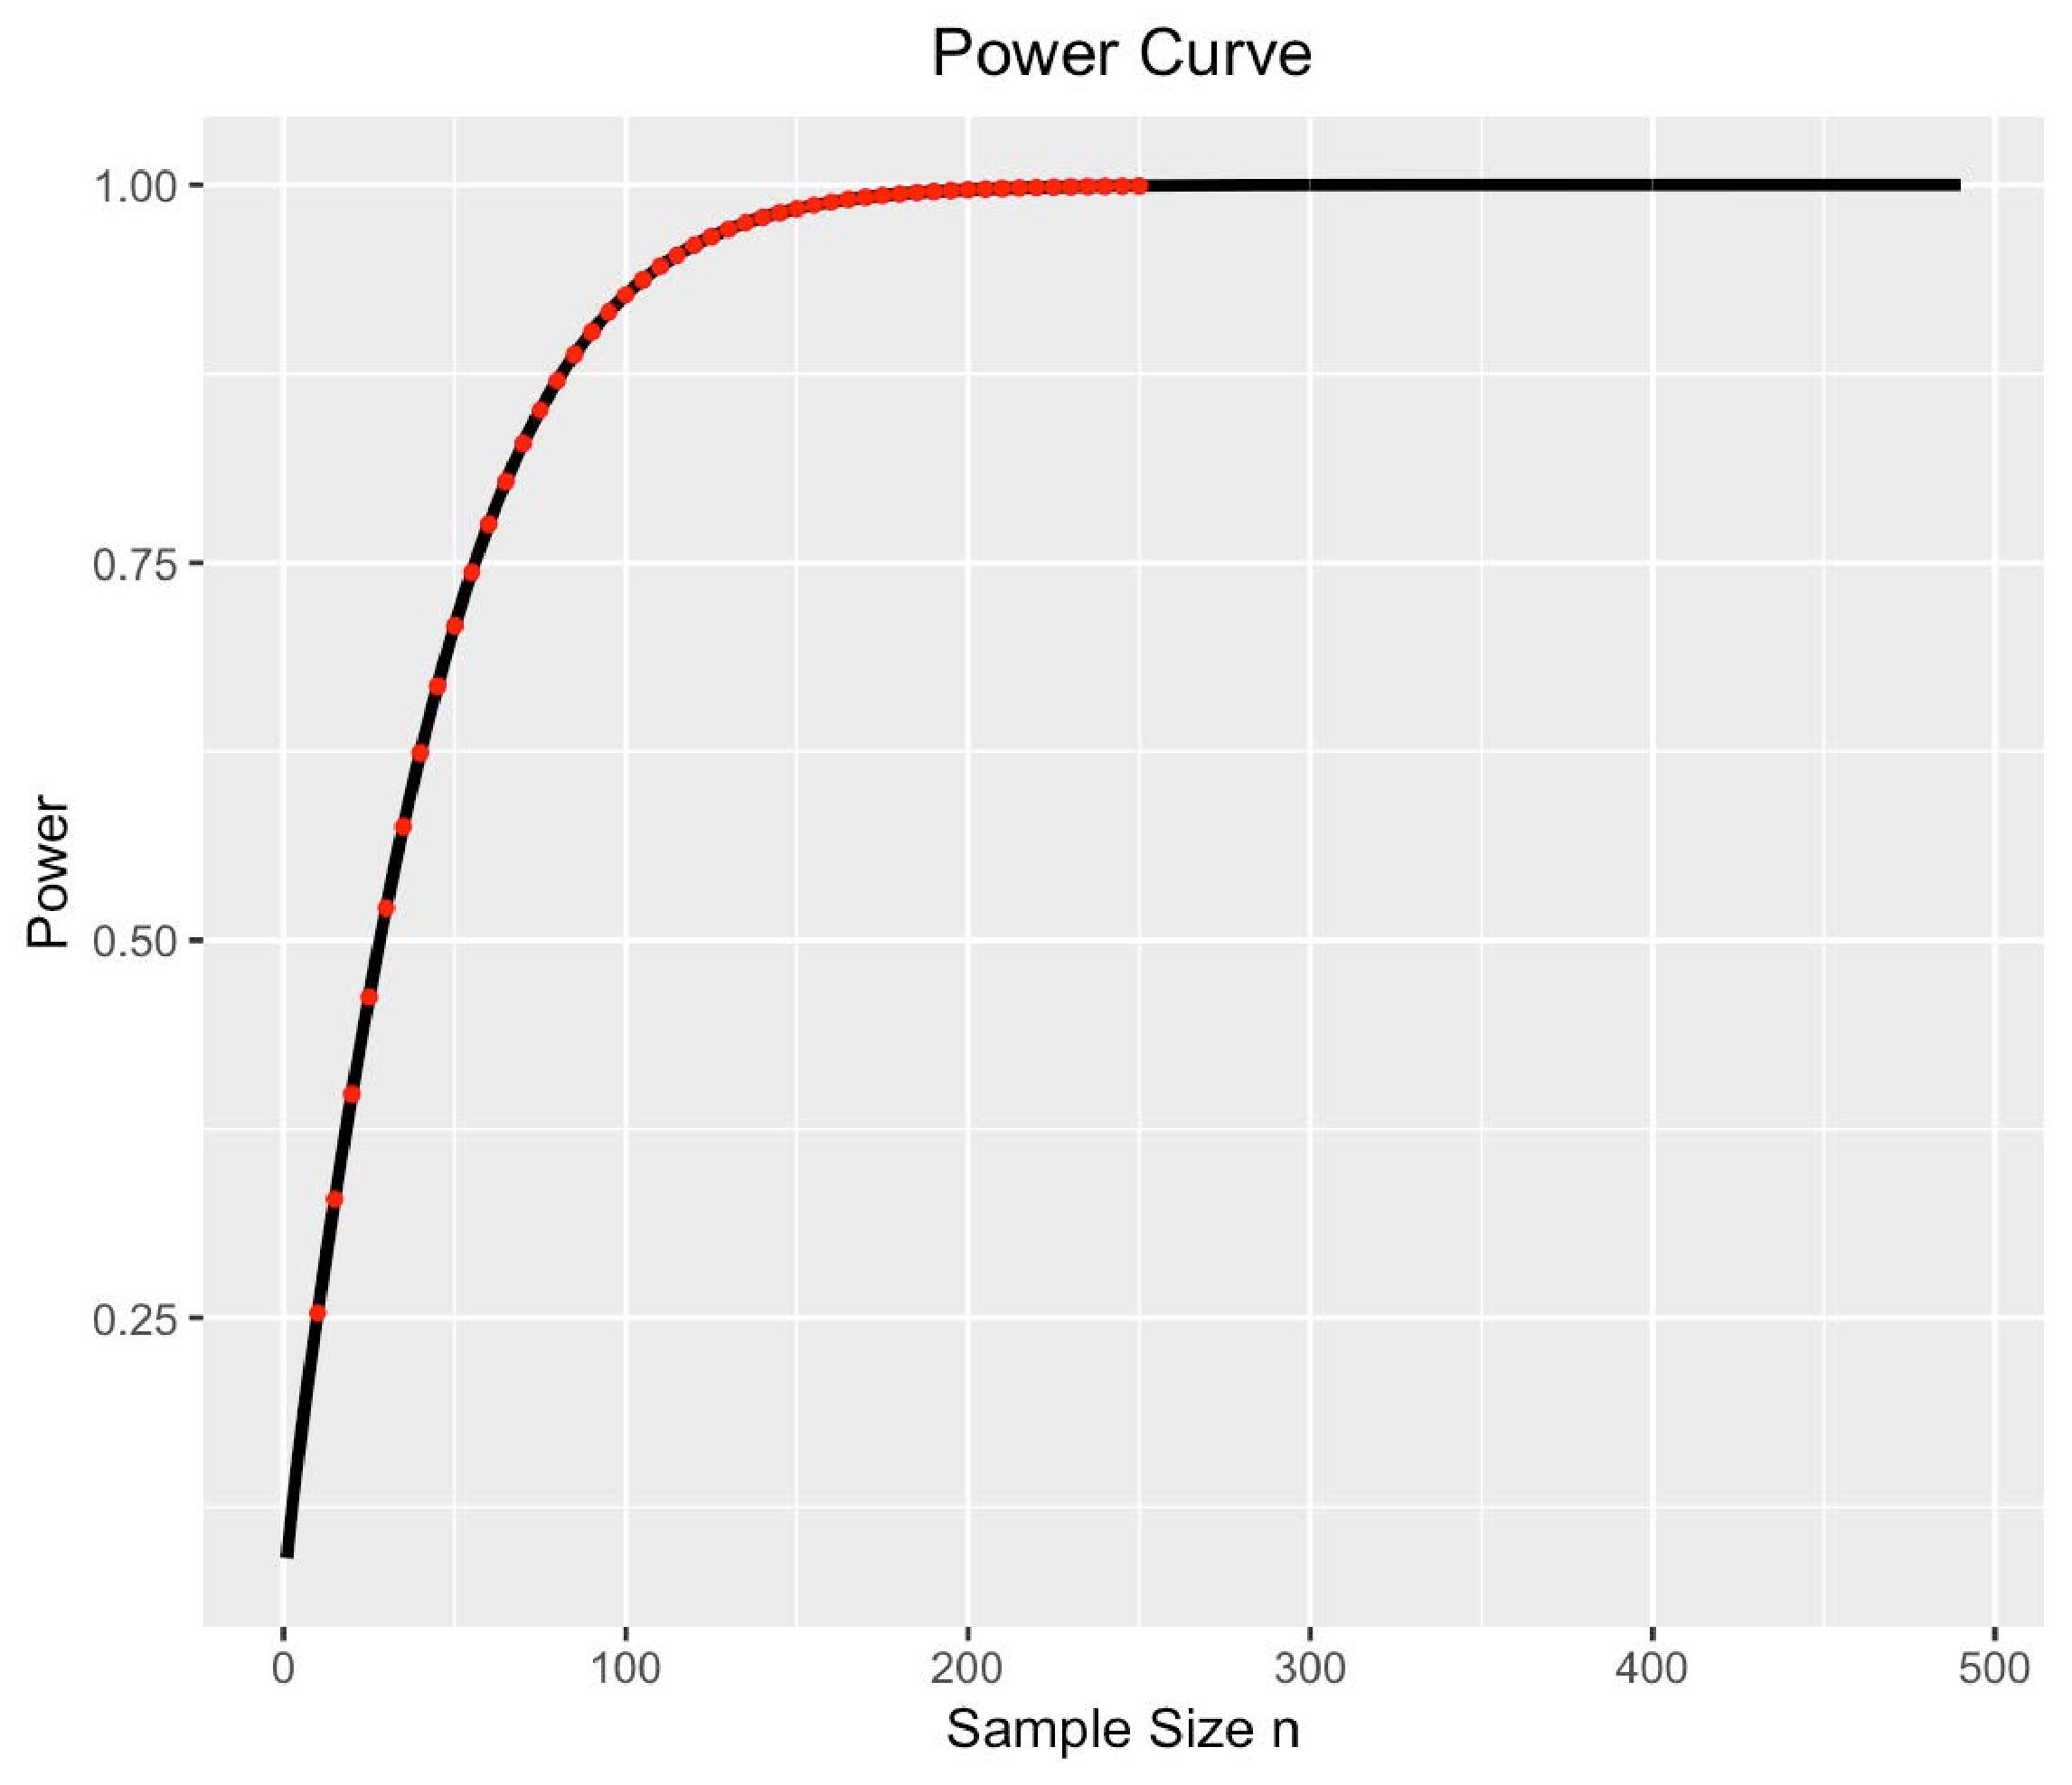
\includegraphics[width=6cm]{pwr_freq_plot.pdf} }}%
    \qquad
    \subfloat[\centering Assurance curve]{{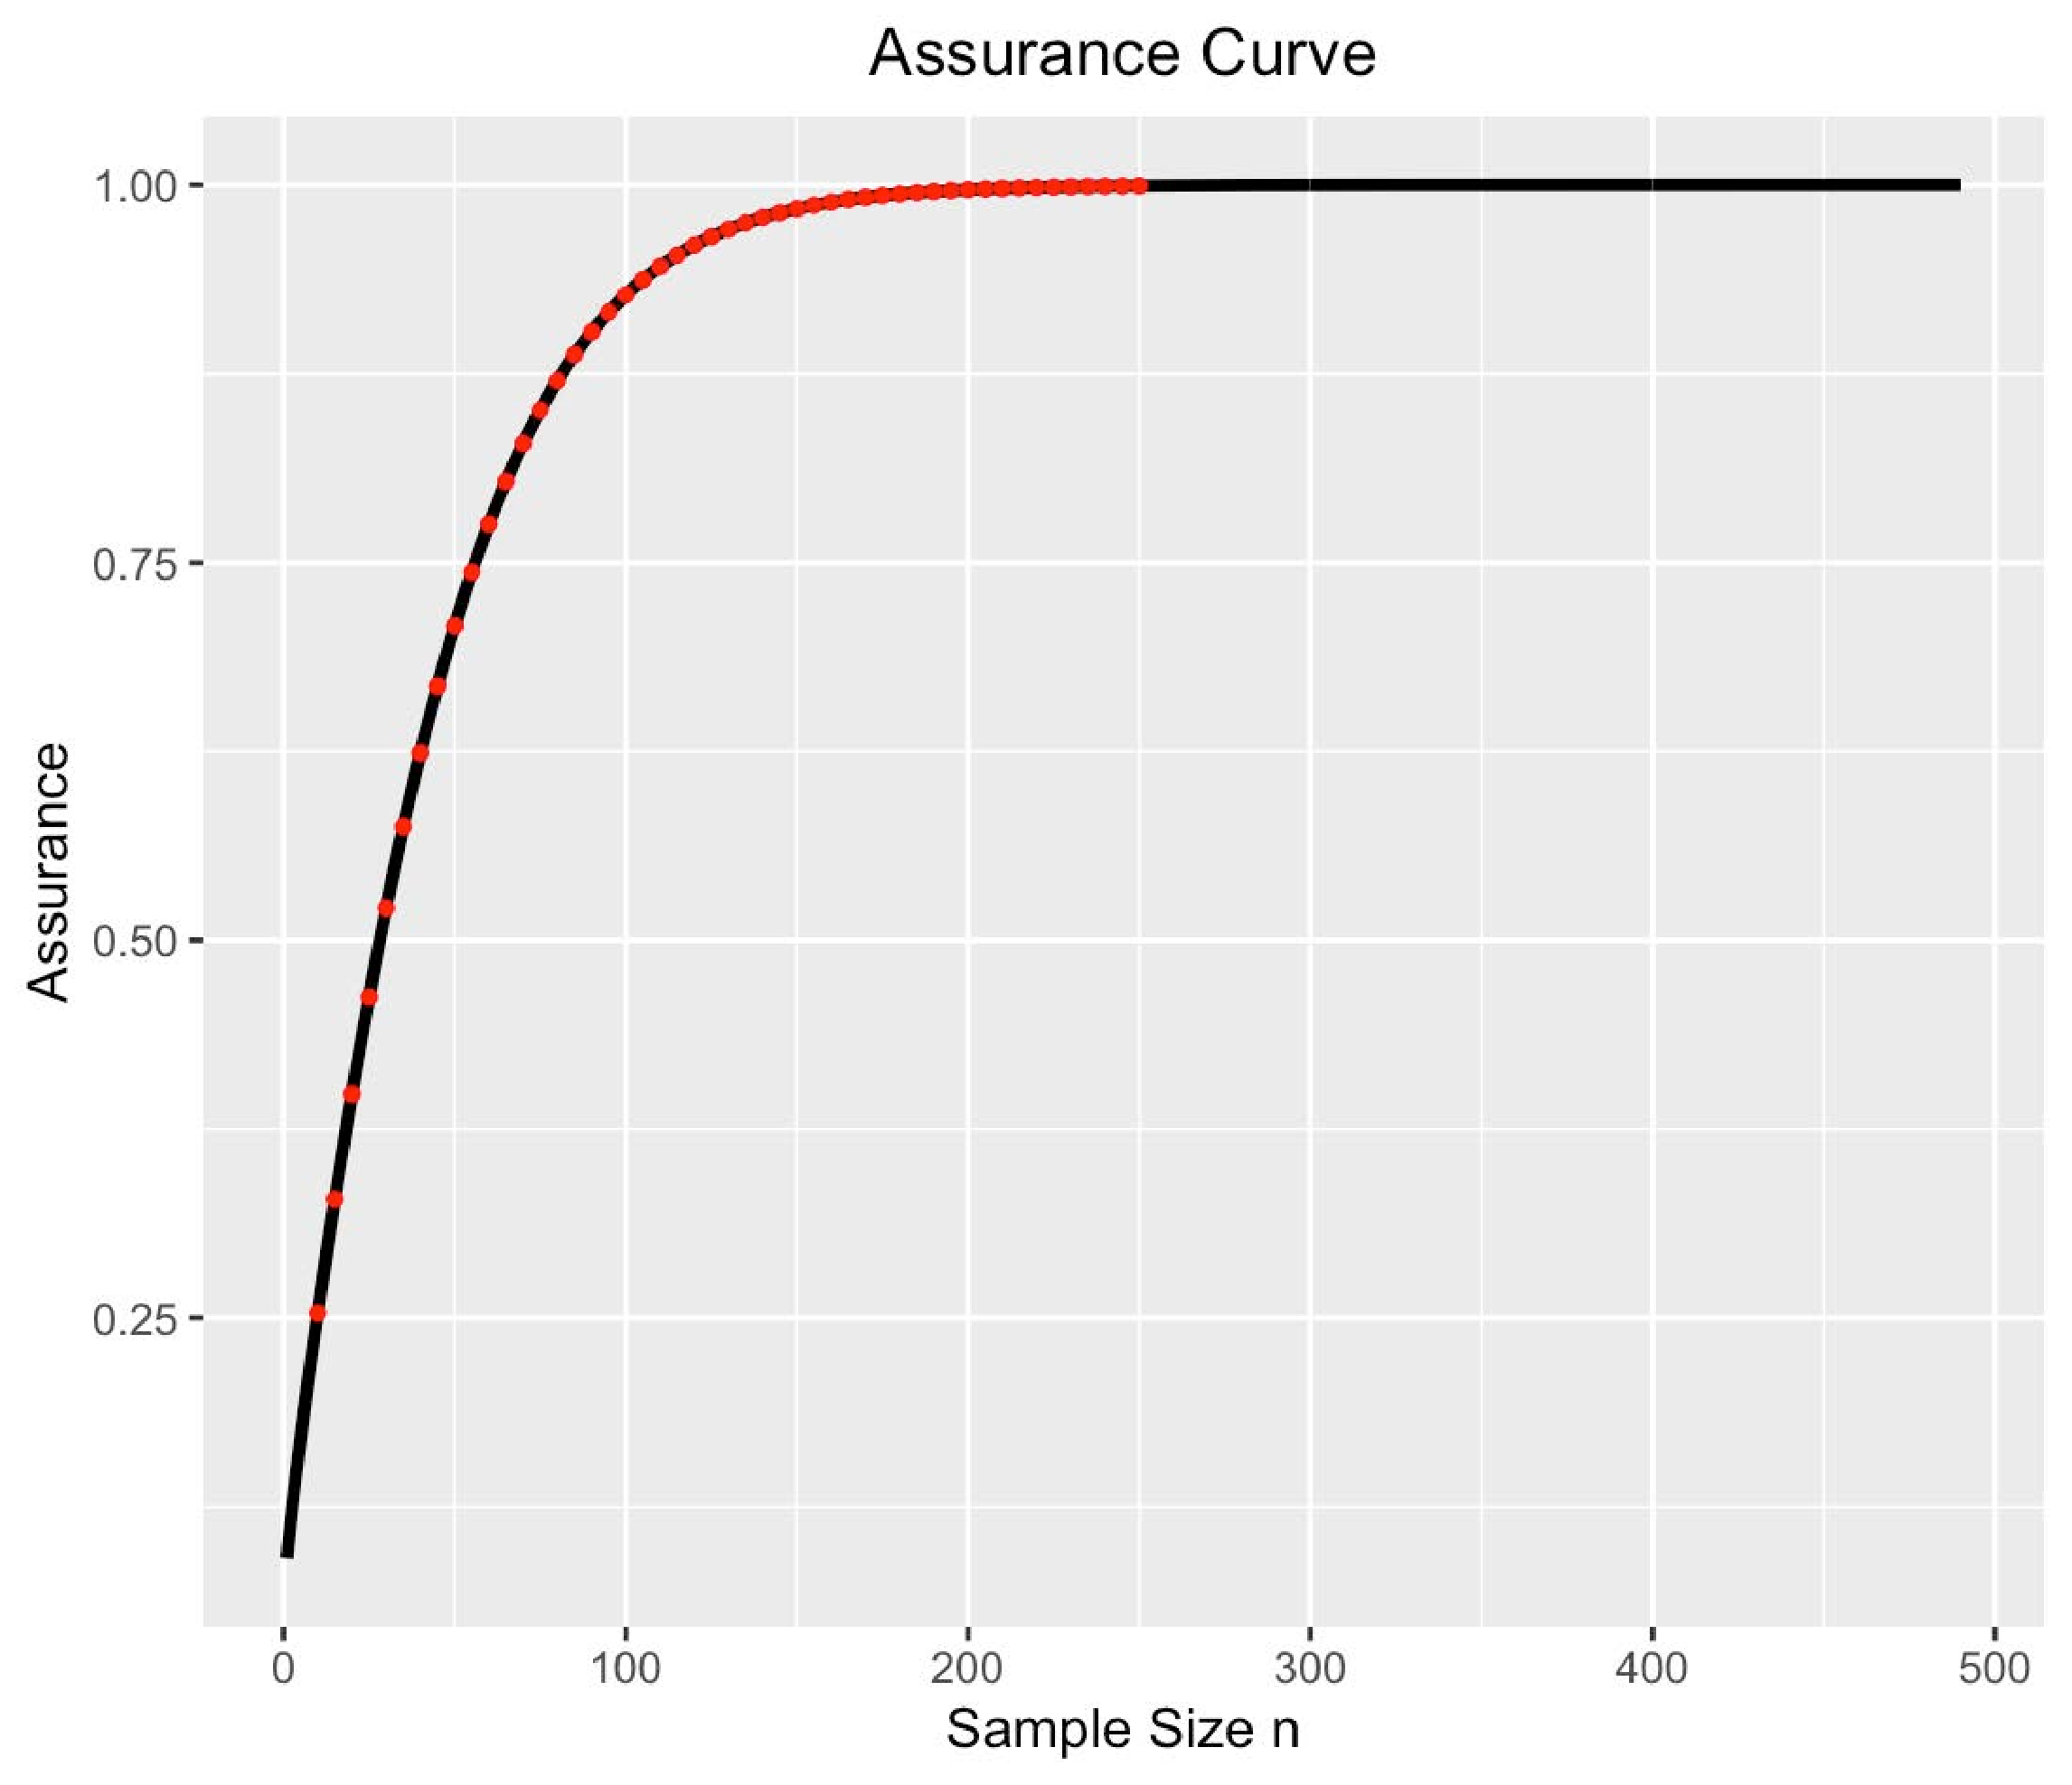
\includegraphics[width=6cm]{assur_plot_simple.pdf} }}%
    \caption{Power and assurance curves are identical when the design priors are strong and the analysis priors are weak.}%
    \label{fig:pwr_assur_curve}%
\end{figure}




\section{Simulation-based functions using conjugate linear models}\label{sec:simform}

Henceforth, we focus on computing 
%The functions discussed in the next several sections 
%determine 
assurance through simulation-based means 
and highlight the common scenario of performing sample 
size analysis where closed-form solutions 
are unavailable. 
%In Sections~\ref{sec:simform} and~\ref{sec:othermethods}, 
In the following sections, we extend upon the 
two-stage design structure 
%briefly mentioned in 
%Section~\ref{sec:closedformassurance} and 
%that frames an outcome to be evaluated in our 
%Monte Carlo-generated samples.  
%and delineate the various conditions addressed in each 
%of the functions and 
and discuss how the design and analysis objectives are 
constructed based on the sample size criteria. 
%Section~\ref{sec:simform}, in particular, draws attention to simulations set within the conjugate Bayesian linear model framework, while Section 4 addresses conditions delineated in other settings.

We seek to evaluate the tenability of a  well-defined analysis
objective using our simulation-based functions. The functions take an iterative approach alternating between generating a dataset in the design stage and evaluating whether or not the dataset satisfies the analysis objective. The assurance equates to the proportion of datasets that meet the objective. 

%To elaborate on this idea in greater detail, 
We start in the analysis stage.
% and frame the condition that
%is to be observed. 
Consider a set of $n$ observations denoted by 
$y = (y_1, y_2, \cdots, y_n)^{\top}$ that are to be collected
together with $p$ controlled explanatory variables,
$x_1, x_2, \cdots, x_p$. Specifically,
\[y = X_n\beta + \epsilon_n,\] 
where $X_n$ is an $n \times p$ design matrix whose $i$th row 
$x_i^{\top}$, and $\epsilon_n \sim N(0, \sigma^2V_n)$, 
where $V_n$ is a known $n \times n$ correlation matrix. 
We assume $X_n$ has linearly independent columns. 
A conjugate Bayesian linear regression model specifies the
joint distribution of the parameters $\{\beta, \sigma^2\}$
and $y$ as 
\[
IG(\sigma^2|a_{\sigma}, b_{\sigma}) \times N(\beta|\mu_{\beta}^{(a)},
\sigma^2V_{\beta}^{(a)}) \times N(y | X_n\beta, \sigma^2V_n),
\]
where superscripts $(a)$ indicate parameters in the analysis stage. 
The objective is to find  
the assurance of the realized 
data favoring $H: u^{\top}\beta > C$, where $u$ is a 
$p \times 1$ vector of fixed contrasts and $C$ is a known constant. 
Inference proceeds from the posterior 
distribution given by 
\begin{equation}
\label{eq:post_dist}
p(\beta, \sigma^2|y) = IG(\sigma^2|a_{\sigma}^*, b_{\sigma}^*)
\times N(\beta|M_nm_n, \sigma^2M_n),
\end{equation}
where 
\begin{align*}
    & M_n^{-1} = V_{\beta}^{-1(a)} + X_n^{\top}V_n^{-1}X_n; \quad m_n = V_{\beta}^{-1(a)}\mu_{\beta}^{(a)} + X_n^{\top}V_n^{-1}y \\
    & a^*_{\sigma} = a_{\sigma}+\frac{n}{2}; \quad 
    b^*_{\sigma} = b_{\sigma} +
    \frac{1}{2}\left\{\mu_{\beta}^{\top}V_{\beta}^{-1}\mu_{\beta} +
    y_n^{\top}V_n^{-1}y - m_n^{\top}M_nm_n\right\}.
\end{align*}
%$a^*_{\sigma} = a_{\sigma}+\frac{n}{2}$, $b^*_{\sigma} = b_{\sigma} + \frac{1}{2}\left\{\mu_{\beta}^{\top}V_{\beta}^{-1}\mu_{\beta} + y_n^{\top}V_n^{-1}y - m_n^{\top}M_nm_n\right\}$, $M_n^{-1} = V_{\beta}^{-1(a)} + X_n^{\top}V_n^{-1}X_n$ and $m_n = V_{\beta}^{-1(a)}\mu_{\beta}^{(a)} + X_n^{\top}V_n^{-1}y$.
The posterior distribution helps shape our
analysis objective. 

If $\sigma^2$ is known and fixed, then the posterior distribution of 
$\beta$ is $\displaystyle p(\beta | \sigma^2, y) = N(\beta | 
M_nm_n, \sigma^2M_n)$ shown
in the Equation~\eqref{eq:post_dist}. 
We use the posterior components
of $\beta$ to evaluate $H: u^{\top}\beta > C$,
where standardization leads to
\begin{equation} \label{eq1}                                                                    
\left.\frac{u^{\top}\beta - u^{\top}M_nm_n}{\sigma \sqrt{u^{\top}M_nu}} \right| \sigma^2, y \sim N(0,1)\;.
\end{equation}
Hence, to assess the tenability of $H: u^{\top}\beta > C$, we decide 
in favor of $H$ if the observed data belongs in the set
\begin{align*}
    A_{\alpha}(u, \beta, C) &= \left\{y: P\left(u^{\top}\beta
    \leq C | y\right)  < \alpha\right\} = \left\{y: \Phi
    \left(\frac{C - u^{\top}M_n m_n}{\sigma \sqrt{u^{\top}M_nu}}\right)
    < \alpha \right\}.
\end{align*}
This defines our analysis objective, which we 
will monitor within each sample iteration. 
Sample generation is taken to account for in the design stage 
discussed in the next section. 

In the design stage, the goal is to seek a 
sample size $n$ such that the
analysis objective is met at least $100\delta \%$ of the time,
where $\delta$ is the assurance.
This step requires determining the marginal 
distribution of $y$, which is assigned a separate set 
of priors to quantify our belief about the population 
from which the sample will be taken. Hence, the marginal 
of $y$ under the design priors will be derived from 
\begin{align}\label{eq: ohagan_stevens_linear_regression_design_priors}
  y &=  X_n\beta + \epsilon_n; \quad \epsilon_n \sim N(0, \sigma^2 V_n)\;;\quad \beta = \mu_{\beta}^{(d)} + \omega; \quad \omega \sim N(0, \sigma^2 V_{\beta}^{(d)})\;,
\end{align}
where $\beta\sim N(\mu_{\beta}^{(d)},\sigma^2 V_{\beta}^{(d)})$ is the design prior on $\beta$ and $(d)$ denotes parameters
in the design stage. Substituting the equation for $\beta$ into the equation for $y$ 
gives $y = X\mu_{\beta}^{(d)} + (X\omega + \epsilon_n)$ and, hence, 
\[
y \sim N\left(X\mu_{\beta}^{(d)}, \sigma^2V_n^{*}\right) \quad \mbox{ and }\quad 
V_n^{\ast} = \left(XV_{\beta}^{(d)}X^{\top} + V_n\right).
\] 
%where $V_n^{\ast} = \left(XV_{\beta}^{(d)}X^{\top} + V_n\right)$. 

To summarize our simulation strategy for estimating
the Bayesian assurance, we fix sample size $n$ and generate
a sequence of $J$ datasets $y^{(1)}, y^{(2)}, ..., y^{(J)}$.
A Monte Carlo estimate of the Bayesian assurance is
computed as 
\[
\hat{\delta}(n) = \frac{1}{J}\sum_{j=1}^J \mathbb{I}\left(\left\{y^{(j)}:
    \Phi \left(\frac{C - u^{\top}M_n^{(j)}m_n^{(j)}}{\sigma
    \sqrt{u^{\top}M_n^{(j)}u}}\right) < \alpha \right\}\right)\;,
\]
where $\mathbb{I}(\cdot)$ is the indicator function of the
event in its argument, $M_n^{(j)}$ and $m_n^{(j)}$ are the
values of $M_n$ and $m_n$ computed from $y^{(j)}$.




\subsection{Assurance computation with known variance}
\label{sec:assur_knownvar}
The simulation-based function, 
\fct{bayes\_sim}, determines the assurance
within the context of conjugate Bayesian linear regression models
assuming known variance, $\sigma^2$.
The execution of \fct{bayes\_sim} is straightforward. 
An important feature is that users are not required to 
provide their own design matrix,
$X_n$, when executing \fct{bayes\_sim}.
When \code{Xn = NULL}, the function automatically 
constructs an appropriate design matrix based on the
specified sample size(s), using the built-in \fct{gen\_Xn} 
function. 

%The algorithm automatically accommodates for the case, \code{Xn = NULL}, using the built-in function, \fct{gen\_Xn}, which constructs appropriate design matrices based on entered sample size(s). 
Later sections discuss design matrix
generators in greater detail. 
%In fact,
%it is in the users' best interest to avoid providing their own
%design matrices unless the objective is to obtain 
%the assurance for a single case. 
Setting \code{Xn = NULL} facilitates calculation
of assurances across
a vector of sample sizes, where the function sequentially 
updates the design matrix for each unique sample
size undergoing evaluation. Table~\ref{tab:bayes_sim} 
lists the required set of parameters. 

\begin{table}[t!]
    \centering
    \begin{tabular}{|p{3cm}||p{8.5cm}|}
    \hline
    \multicolumn{2}{|l|}{\fct{bayes\_sim:} \textbf{Parameters}}\\
    \hline
    \hline
    Variable  & Description \\ 
    \hline
    \hline
     \code{n} & Sample size (either vector or scalar). 
     If vector, each value corresponds to a separate study design. \\
     \hline
     \code{p} & Number of explanatory variables being considered.
     Also denotes the column dimension of design matrix \code{Xn}. 
     If \code{Xn = NULL}, \code{p} must be specified for the 
     function to assign a default design matrix for \code{Xn}. \\
     \hline
     \code{u} & a scalar or vector included in the expression 
     to be evaluated, e.g. $u^{\top}\beta > C$, where $\beta$ 
     is an unknown parameter that is to be estimated. \\
     \hline
     \code{C} & constant to be compared to \\
     \hline
     \code{Xn} & design matrix characterizing the
     observations given by the normal linear regression model 
     $y_n = X_n\beta + \epsilon_n$, where $\epsilon_n \sim 
     N(0, \sigma^2V_n)$. See above description for details. 
     Default \code{Xn} is an $np \times p$ matrix comprised of $n \times 1$ 
     ones vectors that run across the diagonal of the matrix. \\
     \hline
     \code{Vbeta\_d} & correlation matrix that characterizes prior
     information on $\beta$ in the design stage, i.e. $\beta \sim
     N(\mu_{\beta}^{(d)}, \sigma^2 V_{\beta}^{(d)})$. \\
     \hline
     \code{Vbeta\_a\_inv} & inverse-correlation matrix that
     characterizes prior information on $\beta$ in the analysis stage, i.e. 
     $\beta \sim N(\mu_{\beta}^{(a)}, \sigma^2V_{\beta}^{(a)})$. 
     The inverse is passed in for computation efficiency, i.e. $V_{\beta}^{-1(a)}$. \\
     \hline
     \code{Vn} & an $n \times n$ correlation matrix for the marginal
     distribution of the sample data $y_n$. Takes on an identity matrix 
     when set to \code{NULL}. \\
     \hline
     \code{sigsq} & a known and fixed constant preceding all
     correlation matrices \code{Vn}, \code{Vbeta\_d} and
     \code{Vbeta\_a\_inv}. \\
     \hline
     \code{mu\_beta\_d} & design stage mean, $\mu_{\beta}^{(d)}$ \\
     \hline
     \code{mu\_beta\_a} & analysis stage mean, $\mu_{\beta}^{(a)}$ \\
     \hline
     \code{alt} & specifies alternative test case, where 
     \code{alt = "greater"} tests if $u^{\top}\beta > C$,
     \code{alt = "less"} tests if $u^{\top}\beta < C$, and 
     \code{alt = "two.sided"} performs a two-sided test for
     $u^{\top}\beta \neq C$. By default, \code{alt = "greater"}. \\
     \hline
     \code{alpha} & significance level \\
     \hline
     \code{mc\_iter} & number of MC samples evaluated under the analysis objective \\
    \hline
    \end{tabular}
    \caption{Parameter specifications needed to run \fct{bayes\_sim}.}
    \label{tab:bayes_sim}
\end{table}


\subsubsection{Example 1: scalar parameter}

This example computes the 
tenability of $H: u^{\top}\beta > C$ in the case when
$\beta$ is a scalar. In the following code block, we assign 
a set of values for the parameters of 
\fct{bayes\_sim} and saves the outputs as \code{assur\_vals}.
The first ten rows of the table is shown. 
\begin{Schunk}
\begin{Sin}
R> library(bayesassurance)
R> n <- seq(100, 300, 10)
R> assur_vals <- bayes_sim(n, p = 1, u = 1,
      C = 0.15, Xn = NULL, Vbeta_d = 0, Vbeta_a_inv = 0,
      Vn = NULL, sigsq = 0.265, mu_beta_d = 0.25, mu_beta_a = 0,
      alt = "greater", alpha = 0.05, mc_iter = 5000)

R> head(assur_vals$assurance_table)
R> assur_vals$assurance_plot

\end{Sin}
\begin{Sout}
   Observations per Group (n) Assurance
1                         100    0.6162
2                         110    0.6612
3                         120    0.6886
4                         130    0.7148
5                         140    0.7390
6                         150    0.7746
\end{Sout}
\end{Schunk}

%We emphasize a few important points in this  rudimentary example. A vector of values for \code{n} indicates we are interested in assessing the assurance for multiple study designs. 
Each unique value passed into \code{n} corresponds to a separate balanced study design
containing that particular sample size for each of the $p$ groups undergoing assessment. In this example, setting \code{p = 1}, \code{u = 1} and \code{C = 0.15} implies that we are evaluating the tenability of $H: \beta > 0.15$, where $\beta$ is a scalar. Furthermore, \code{Vbeta\_d} and \code{Vbeta\_a\_inv} are scalars to align 
with the dimension of $\beta$. A weak analysis prior (\code{Vbeta\_a\_inv = 0}) and a strong design prior (\code{Vbeta\_d = 0}) produces the classical power analysis. 
We revisit this example in a later section when
reviewing features that allow users to simultaneously visualize the Bayesian and frequentist power analyses. Finally, \code{Xn} and \code{Vn} are set to \code{NULL}, which means they will take on the default settings described above. 

\subsubsection{Example 2: linear contrasts}
\label{subsec:ex2}

In this example, we assume $\beta$ is a vector of unknown components rather than a scalar. We use
the real-world example discussed in~\cite{ohagan}. Specifically, we consider 
a randomized clinical trial  that compares the cost-effectiveness of two treatments.
Cost-effectiveness is evaluated using
a net monetary benefit measure expressed as
\[
\xi = K(\mu_2 - \mu_1) - (\gamma_2 - \gamma_1),
\]
where $\mu_1$ and $\mu_2$ denote the efficacy of treatments 1 and 2, and $\gamma_1$ and $\gamma_2$ denote the costs, respectively. 
Hence, $\mu_2 - \mu_1$ and $\gamma_2 - \gamma_1$
correspond to the true differences in 
treatment efficacy and costs.
%, respectively, between treatments 1 and 2. 
The threshold unit cost, $K$, represents the maximum price that a 
health care provider is willing to pay for a 
unit increase in efficacy. 

In this setting,we seek the tenability of $H: \xi > 0$, which, if true, indicates that treatment~2 is more cost-effective than treatment~1. To comply with the conjugate linear model framework outlined in \eqref{eq:post_dist}, we set 
$u = (-K, 1, K, -1)^{\top}$, $\beta = (\mu_1, \gamma_1, \mu_2, \gamma_2)^{\top}$, and $C = 0$, giving us an equivalent form of $\xi > 0$ expressed as  $u^{\top}\beta > 0$. All other inputs of this application were directly pulled from \cite{ohagan}. The following code sets up the inputs to be passed into \fct{bayes\_sim}. 

\begin{Schunk}
\begin{Sin}

R> n <- 285
R> p <- 4
R> K <- 20000 # threshold unit cost
R> C <- 0
R> u <- as.matrix(c(-K, 1, K, -1))
R> sigsq <- 4.04^2

## Assign mean parameters to analysis and design stage priors
R> mu_beta_d <- as.matrix(c(5, 6000, 6.5, 7200))
R> mu_beta_a <- as.matrix(rep(0, p))

## Assign correlation matrices (specified in paper) 
## to analysis and design stage priors
R> Vbeta_a_inv <- matrix(rep(0, p^2), nrow = p, ncol = p)
R> Vbeta_d <- (1 / sigsq) * matrix(c(4, 0, 3, 0, 0, 10^7, 0, 
    0, 3, 0, 4, 0, 0, 0, 0, 10^7), nrow = 4, ncol = 4)

R> tau1 <- tau2 <- 8700
R> sig <- sqrt(sigsq)
R> Vn <- matrix(0, nrow = n*p, ncol = n*p)
R> Vn[1:n, 1:n] <- diag(n)
R> Vn[(2*n - (n-1)):(2*n), (2*n - (n-1)):(2*n)] <- (tau1 / sig)^2 * diag(n)
R> Vn[(3*n - (n-1)):(3*n), (3*n - (n-1)):(3*n)] <- diag(n)
R> Vn[(4*n - (n-1)):(4*n), (4*n - (n-1)):(4*n)] <- (tau2 / sig)^2 * diag(n)

\end{Sin}
\end{Schunk}

The inputs specified above should result in 
an assurance of approximately 0.70 according to
~\cite{ohagan}. The \fct{bayes\_sim}
returns a similar value, demonstrating
that sampling from the posterior yields results similar to those reported in the paper. 

\begin{Schunk}
\begin{Sin}

R> library(bayesassurance)

R> assur_vals <- bayes_sim(n = 285, p = 4,  u = as.matrix(c(-K, 1, K, -1)), 
   C = 0, Xn = NULL, Vbeta_d = Vbeta_d,Vbeta_a_inv = Vbeta_a_inv, 
   Vn = Vn, sigsq = 4.04^2, mu_beta_d = as.matrix(c(5, 6000, 6.5, 7200)), 
   mu_beta_a = as.matrix(rep(0, p)),  alt = "greater", alpha = 0.05, mc_iter = 10000)
   
R> assur_vals

\end{Sin}
\begin{Sout}
## [1] "Assurance: 0.722"
\end{Sout}
\end{Schunk}




\subsection{Assurance computation in the longitudinal setting}
\label{sec:assur_longitudinal}
We demonstrate an additional feature embedded in the function tailored to longitudinal data.  In this setting, $n$ no longer refers to the number of subjects but rather the number of repeated measures reported for each subject, assuming a balanced study design.  Referring back to the linear regression model discussed in the general framework,  we can construct a longitudinal model that utilizes this same linear regression form, where $y_n = X_n\beta + \epsilon_n$.

Consider a group of subjects in a balanced longitudinal study with the same number of repeated measures at  equally-spaced time points.  In the base case, where time is treated as a linear term, subjects can be characterized as
\[
%y_{ij} = \beta_{0i} + \beta_{1i}t_{ij} + \epsilon_{ij}, 
y_{ij} = \alpha_{i} + \beta_{i}t_{ij} + \epsilon_{i}, 
\]
where $y_{ij}$ denotes the $j^{th}$ observation on subject $i$ at time $t_{ij}$, $\alpha_{i}$ and $\beta_{i}$ denote the intercept and slope terms for subject $i$, respectively, and $\epsilon_i \sim N(0, \sigma^2_i)$ is an error term. 

In a simple case with two subjects, we can individually  express the observations as
\begin{align*}
y_{11} &= \alpha_{1} + \beta_{1}t_{11} + \epsilon_{1}\\
&\vdots\\
y_{1n} &= \alpha_{1} + \beta_{1}t_{1n} + \epsilon_{1}\\
y_{21} &= \alpha_{2} + \beta_{2}t_{21} + \epsilon_{2}\\
&\vdots\\
y_{2n} &= \alpha_{2} + \beta_{2}t_{2n} + \epsilon_{2},
\end{align*}
assuming that each subject contains $n$ observations. The model can also be expressed using matrices:
\begin{gather}
\label{eq:long_model}
 \underbrace{\begin{pmatrix} y_{11} \\ \vdots \\ y_{1n} \\ y_{21} \\ \vdots\\ y_{2n} \end{pmatrix}}_{y_n} =
   \underbrace{
   \begin{pmatrix}
   1 & 0 & t_{11} & 0\\
   \vdots & \vdots & \vdots & \vdots \\
   1 & 0 & t_{1n} & 0\\
   0 & 1 & 0 & t_{21}\\
   \vdots & \vdots & \vdots & \vdots \\
   0 & 1 & 0 & t_{2n}
   \end{pmatrix}
   }_{X_n}
   \underbrace{
      \begin{pmatrix}
         \alpha_{1}\\
         \alpha_{2}\\
         \beta_{1}\\
         \beta_{2}
      \end{pmatrix}
   }_{\beta}
   + 
   \underbrace{
   \begin{pmatrix}
   \epsilon_{1}\\
   \vdots\\
   \epsilon_{1}\\
   \epsilon_{2}\\
   \vdots\\
   \epsilon_{2}
   \end{pmatrix}
   }_{\epsilon_n}
\end{gather}
bringing us back to the linear model structure. If higher degrees are to be considered for the time variable, such as the inclusion of a quadratic term, the model would be altered to include additional covariate terms that can accommodate these changes. In the two-subject case,  incorporating a quadratic term for the time variable in \eqref{eq:long_model} will result in the model being modified as follows: 
\begin{gather}
\nonumber
 \underbrace{\begin{pmatrix} y_{11} \\ \vdots \\ y_{1n} \\ y_{21} \\ \vdots\\ y_{2n} \end{pmatrix}}_{y_n} =
   \underbrace{
   \begin{pmatrix}
   1 & 0 & t_{11} & 0 & t_{11}^2 & 0\\
   \vdots & \vdots & \vdots & \vdots & \vdots & \vdots\\
   1 & 0 & t_{1n} & 0 & t_{1n}^2  & 0\\
   0 & 1 & 0 & t_{21} & 0 & t_{21}^2 \\
   \vdots & \vdots & \vdots & \vdots & \vdots & \vdots \\
   0 & 1 & 0 & t_{2n} & 0 & t_{2n}^2
   \end{pmatrix}
   }_{X_n}
   \underbrace{
      \begin{pmatrix}
         \alpha_{1}\\
         \alpha_{2}\\
         \beta_{1}\\
         \beta_{2}\\
         \phi_{1}\\
         \phi_{2}
      \end{pmatrix}
   }_{\beta}
   + 
   \underbrace{
   \begin{pmatrix}
   \epsilon_{1}\\
   \vdots\\
   \epsilon_{1}\\
   \epsilon_{2}\\
   \vdots\\
   \epsilon_{2}
   \end{pmatrix}
   }_{\epsilon_n}
\end{gather}
In general, for $m$ subjects who each have
$n$ repeated measures, a one-unit increase in the degree of the time-based covariate will
result in $m$ additional columns being added to the  design matrix $X_n$ and $m$ additional rows added to the $\beta$ vector. 

When working in the longitudinal setting,
additional parameters need to be specified
in the \fct{bayes\_sim} function, which can 
be found in Table~\ref{tab:long}.
\begin{table}[t!]
    \centering
    \begin{tabular}{|p{4.5cm}||p{8.5cm}|}
    \hline
    \multicolumn{2}{|l|}{\fct{bayes\_sim}: \textbf{Additional Parameters used in the Longitudinal Setting}}\\
    \hline
    \hline
    Variable  & Description \\ 
    \hline
    \hline
     \code{longitudinal} & logical that 
     indicates the simulation will be based in a longitudinal setting. 
     If \code{Xn = NULL}, the function will construct a design 
     matrix using inputs that correspond to a balanced
     longitudinal study design.\\
     \hline
     \code{ids} & vector of unique subject ids. \\
     \hline
     \code{from} & start time of repeated measures for each subject\\
     \hline
     \code{to} & end time of repeated measures for each subject \\
     \hline
     \code{num\_repeated\_measures} & desired length of 
     the repeated measures sequence.This should be a non-negative
     number, will be rounded up otherwise if fractional. \\
     \hline
     \code{num\_repeated\_measures} & desired length of 
     the repeated measures sequence.This should be a non-negative
     number, will be rounded up otherwise if fractional.\\
     \hline
     \code{poly\_degree} & degree of polynomial in longitudinal model, set to 1 by default.\\
     \hline
    \end{tabular}
    \caption{Additional parameter specifications needed to run \fct{bayes\_sim} in 
    the longitudinal setting.}
    \label{tab:long}
\end{table}
By default, \code{longitudinal = FALSE} and \code{ids,
from}, and \code{to} are set to \code{NULL} when
working within the standard conjugate linear model. 
When \code{longitudinal = TRUE}, \code{n} takes on a 
different meaning as its value(s) correspond to the number 
of repeated measures for each subject rather than the 
total number of subjects in each group. 
When \code{longitudinal = TRUE} and \code{Xn = NULL},
\fct{bayes\_sim} implicitly relies on a design matrix generator,
\fct{gen\_Xn\_longitudinal}, that is specific to the longitudinal setting
to construct appropriate design matrices. 
%Section~\ref{sec:tools} discusses this in greater detail. 



\subsubsection{Example 3: longitudinal setting}
The following example uses similar parameter settings as 
the cost-effectiveness example we had previously discussed
in Example 2, 
%in Section~\ref{subsec:ex2},
now with 
longitudinal specifications. We assume two subjects and
want to test whether the growth rate of subject 1
is different from that of subject 2. 
%This could have either positive or negative implications depending on the measurement scale. 
Figure~\ref{fig:ex3} displays the estimated assurance points
given the specifications. 

Assigning an appropriate linear contrast
lets us evaluate the tenability of an outcome. 
Let us consider the tenability of 
$u^{\top}\beta \neq C$ in this next example that uses
simulated data, where
$u = (1, -1, 1, -1)^{\top}$ and $C = 0$. 
There are 120 arbitrary timepoints.
%The timepoints are arbitrarily chosen to be 0 through 120- this could be days, months, or years depending on the context of the problem. 
The number of repeated measurements per subject
to be tested includes values 10 through 100 in increments of 5. 
This indicates that we are evaluating
the assurance for 19 study designs in total. $n = 10$ 
divides the specified time interval 
into 10 evenly-spaced timepoints between 0 and 120.

\begin{figure}[t!]
\centering
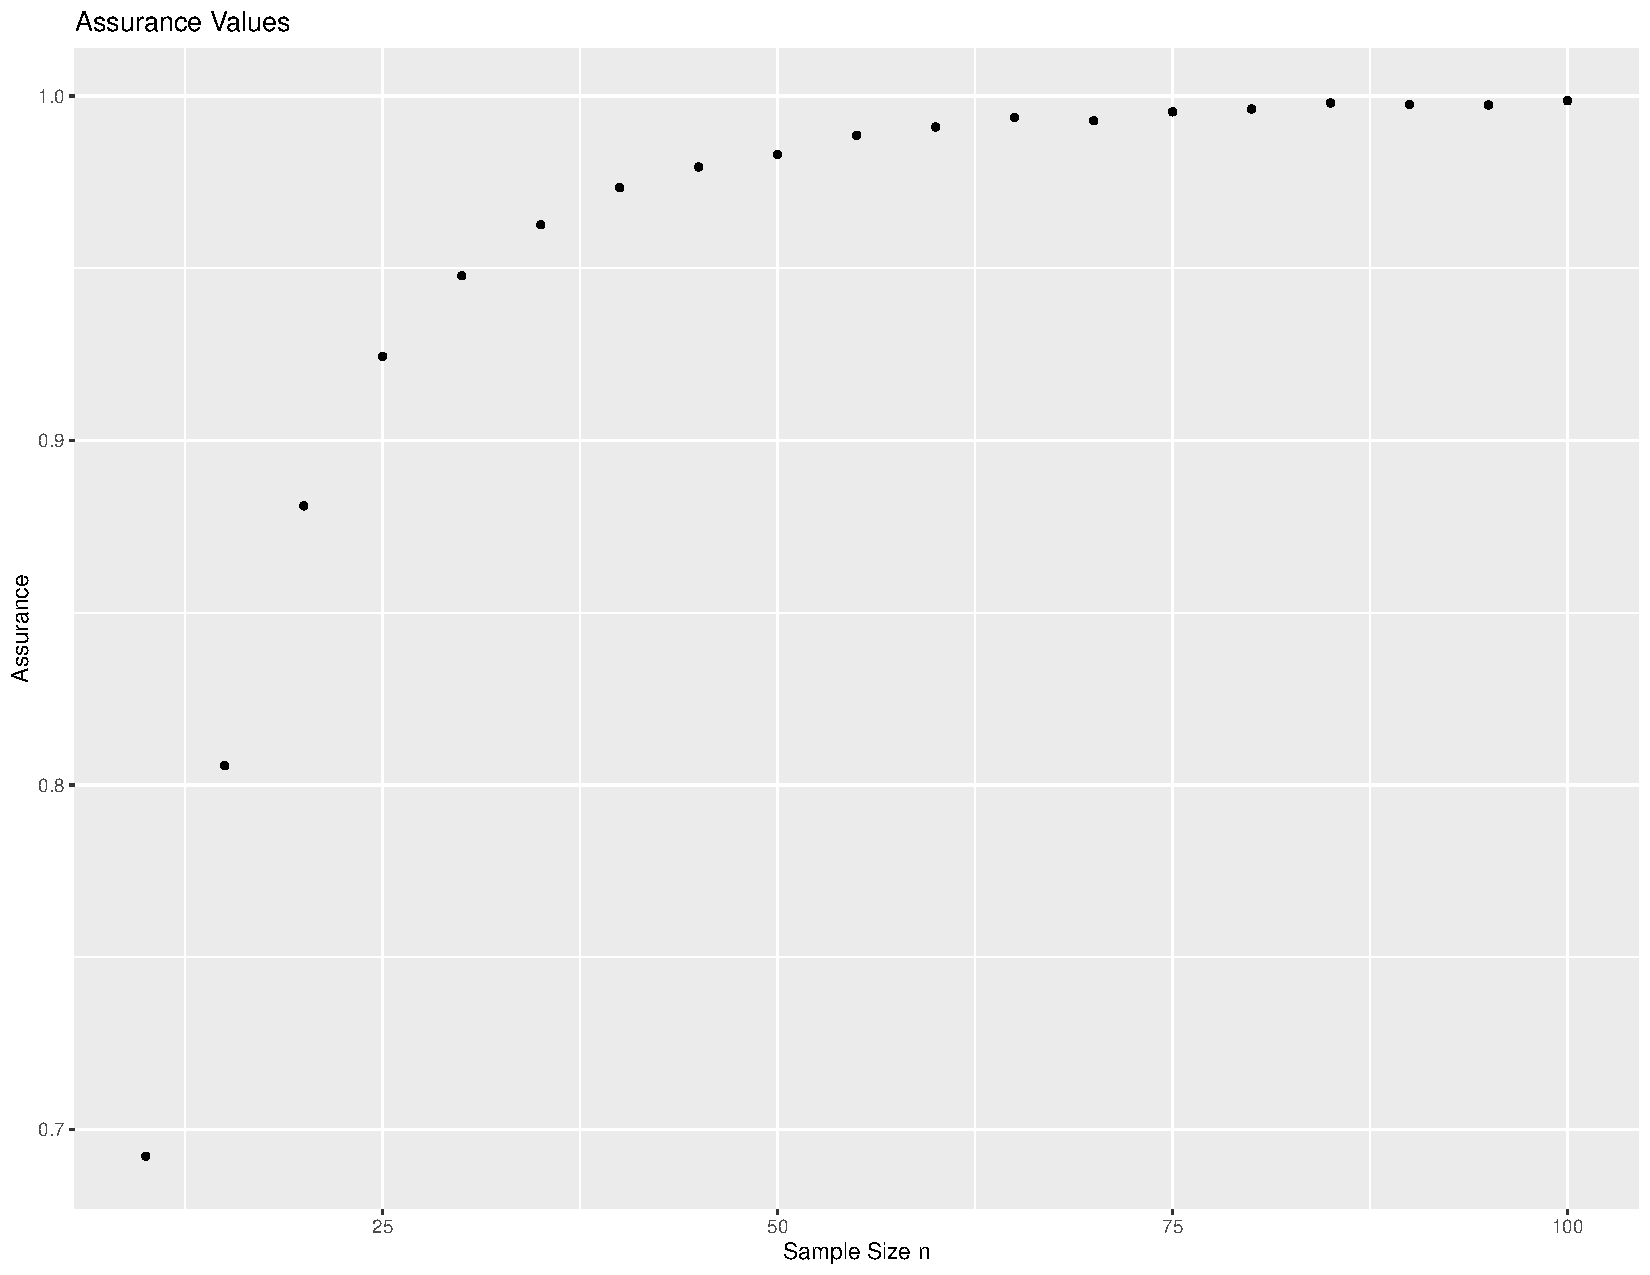
\includegraphics[width = 8 cm]{ex3_assurplot.pdf}
\caption{\label{fig:ex3} Estimated assurance points for longitudinal example.}
\end{figure}

For a more complicated study design comprised of more
than two subjects that are divided into two treatment groups, 
consider testing if the mean growth rate is higher in 
the first treatment group than that of the second, 
e.g. if we have three subjects per treatment group, 
the linear contrast would be set as 
$u = (0, 0, 0, 0, 0, 0, 1/3, 1/3, 1/3, -1/3, -1/3, -1/3)^{\top}$.

\begin{Schunk}
\begin{Sin}
R> n <- seq(10, 100, 5)
R> ids <- c(1,2)
R> Vbeta_a_inv <- matrix(rep(0, 16), nrow = 4, ncol = 4)
R> sigsq <- 100
R> Vbeta_d <- (1 / sigsq) * matrix(c(4, 0, 3, 0, 0, 6, 0, 0, 3, 0, 4, 0, 0, 0, 0, 6), 
                                nrow = 4, ncol = 4)

R> assur_out <- bayes_sim(n = n, p = NULL, u = c(1, -1, 1, -1), C = 0, Xn = NULL,
                       Vbeta_d = Vbeta_d, Vbeta_a_inv = Vbeta_a_inv,
                       Vn = NULL, sigsq = 100,
                       mu_beta_d = as.matrix(c(5, 6.5, 62, 84)),
                       mu_beta_a = as.matrix(rep(0, 4)), mc_iter = 5000,
                       alt = "two.sided", alpha = 0.05, longitudinal = TRUE, ids = ids,
                       from = 10, to = 120)
                       
R> head(assur_out$assurance_table)
R> assur_out$assurance_plot                 
\end{Sin}
\begin{Sout}
  Observations per Group (n) Assurance
1                         10    0.6922
2                         15    0.8056
3                         20    0.8810
4                         25    0.9244
5                         30    0.9478
6                         35    0.9626
\end{Sout}
\end{Schunk}



\subsection{Assurance computation for unbalanced study designs}
\label{sec:assur_unbalanced}

The \fct{bayes\_sim\_unbalanced} function operates similarly to
\fct{bayes\_sim} 
%in Section~\ref{sec:assur_knownvar}
but estimates the assurance of attaining $u^{\top}\beta > C$ 
specifically in unbalanced design settings.
Users provide two sets of sample sizes of equal length,
whose corresponding pairs are considered for  
each study design case. 
%The sample sizes need not be equal to one another, allowing for unbalanced designs. This is unlike \fct{bayes\_sim} that strictly determines assurance for balanced cases, where users specify a single set of sample sizes whose individual entries correspond to a distinct trial comprised of an equal number of observations across all explanatory variables.
%with each individual entry corresponding
The \fct{bayes\_sim\_unbalanced} function provides 
a higher degree of flexibility for designing unbalanced studies
and offers a more advanced visualization feature. Users
have the option of viewing assurance as a 3-D contour 
plot and assess how the assurance behaves
across varying combinations of the two 
sets of sample sizes that run along the 
$x$ and $y$ axes.

The \fct{bayes\_sim\_unbalanced} function is similar to
\fct{bayes\_sim} in terms of parameter specifications with a few
exceptions. Parameters unique to \fct{bayes\_sim\_unbalanced} 
are summarized in Table~\ref{tab:unbalanced}. Here, 
\code{Xn = NULL}, \code{Vn = NULL}, \code{repeats = 1} and \code{surface\_plot = TRUE} by default. 

\begin{table}[t!]
    \centering
    \begin{tabular}{|p{4cm}||p{8.5cm}|}
    \hline
    \multicolumn{2}{|l|}{\fct{bayes\_sim\_unbalanced}: \textbf{Parameters for Unbalanced Study Designs}}\\
    \hline
    \hline
    Variable  & Description \\ 
    \hline
    \hline
     \code{n1} & first sample size (either vector or scalar).\\
     \hline
     \code{n2} & second sample size (either vector or scalar). \\
     \hline
     \code{repeats} & an integer denoting the number of \code{c(n1, n2)} pairs we we are considering. For example, if \code{repeats = 2}, this means we will compute the assurance corresponding to the sample size set of \code{c(n1, n2, n1, n2)}.
     %used in study designs that consider an even number of explanatory variables of at least 2.
     %and whose sample sizes correspond to those specified in \code{n1} and \code{n2}.  
     By default, \code{repeats = 1}. See
     Example 5. \\
     \hline
     \code{surface\_plot} & logical parameter that 
     indicates whether a contour plot is to be constructed. 
     When set to \code{TRUE}, and \code{n1} and \code{n2} are 
     vectors, a contour plot (i.e. heat map) showcasing assurances 
     obtained for all unique combinations of \code{n1} and \code{n2} is produced. \\
     \hline
    \end{tabular}
    \caption{Parameter specifications needed to run \fct{bayes\_sim\_unbalanced}.}
    \label{tab:unbalanced}
\end{table}
As in \code{bayes\_sim}, it is recommended that users 
set \code{Xn = NULL} to facilitate the automatic 
construction of appropriate design matrices that best aligns with
the conjugate linear model. 
%described in beginning of Section~\ref{sec:simform}. 
Recall that every unique sample
size (or sample size pair) passed in corresponds to 
a separate study that requires a separate design matrix. 
Should users choose to provide their own design matrix, 
it is advised that they evaluate the assurance for
one study design at a time,
%the best practice would involve evaluating one study
%design at a time, 
in which a single design matrix is passed
into \code{Xn} along with scalar values assigned for the
sample size parameter(s). 

Saved outputs from executing the function include
\begin{enumerate}
\item{\code{assurance\_table}: table of sample size 
and corresponding assurance values}
\item{\code{contourplot}: contour map of assurance values 
if \code{surface.plot = TRUE}}
\item{\code{mc\_samples}: number of Monte Carlo 
samples that were generated for evaluation}
\end{enumerate}


\subsubsection{Example 4: unbalanced assurance computation with surface plot}

The following code provides a basic example of how
\fct{bayes\_sim\_unbalanced} is executed. It is important to check 
that the parameters passed in are appropriate in dimensions, e.g. 
\code{mu\_beta\_a} and \code{mu\_beta\_d} should each 
contain the same length as that of \code{u}, and the length of 
\code{u} should be equal to the row and column
dimensions of \code{Vbeta\_d} and \code{Vbeta\_a\_inv}.  

A table of assurance values is printed simply
by calling \code{assur\_out\$assurance\_table}, which contains
the exact assurance values corresponding to each
sample size pair. The contour 
plot, shown in Figure~\ref{fig:ex5}, is displayed
using \code{assur\_out\$contourplot}, and offers a visual
depiction of how the assurance varies across unique
combinations of \code{n1} and \code{n2}.  Areas 
with lighter shades denote higher assurance levels.
%No discernible patterns or trends are observed based on  the random behavior of the plot and the proximity of values reported in the table. 
%as the inputs were arbitrarily chosen with no context. 
The next example implements the
function in a real-world setting that offers more sensible
results.
\begin{Schunk}
\begin{Sin}
R> library(bayesassurance)

R> n1 <- seq(20, 75, 5)
R> n2 <- seq(50, 160, 10)


R> assur_out <- bayes_sim_unbalanced(n1 = n1, n2 = n2, repeats = 1, u = c(1, -1),
	  C = 0, Xn = NULL, Vbeta_d = matrix(c(50, 0, 0, 10),nrow = 2, ncol = 2),
	  Vbeta_a_inv = matrix(rep(0, 4), nrow = 2, ncol = 2),
	  Vn = NULL, sigsq = 100,  mu_beta_d = c(1.17, 1.25),
	  mu_beta_a = c(0, 0), alt = "two.sided", alpha = 0.05, mc_iter = 5000,
	  surface_plot = TRUE)
				
R> head(assur_out$assurance_table)
R> assur_out$contourplot 

\end{Sin}
\begin{Sout}
  n1  n2 Assurance
1 20  50    0.9504
2 25  60    0.9584
3 30  70    0.9508
4 35  80    0.9616
5 40  90    0.9624
6 45 100    0.9634
\end{Sout}
\end{Schunk}

\begin{figure}[t!]
\centering
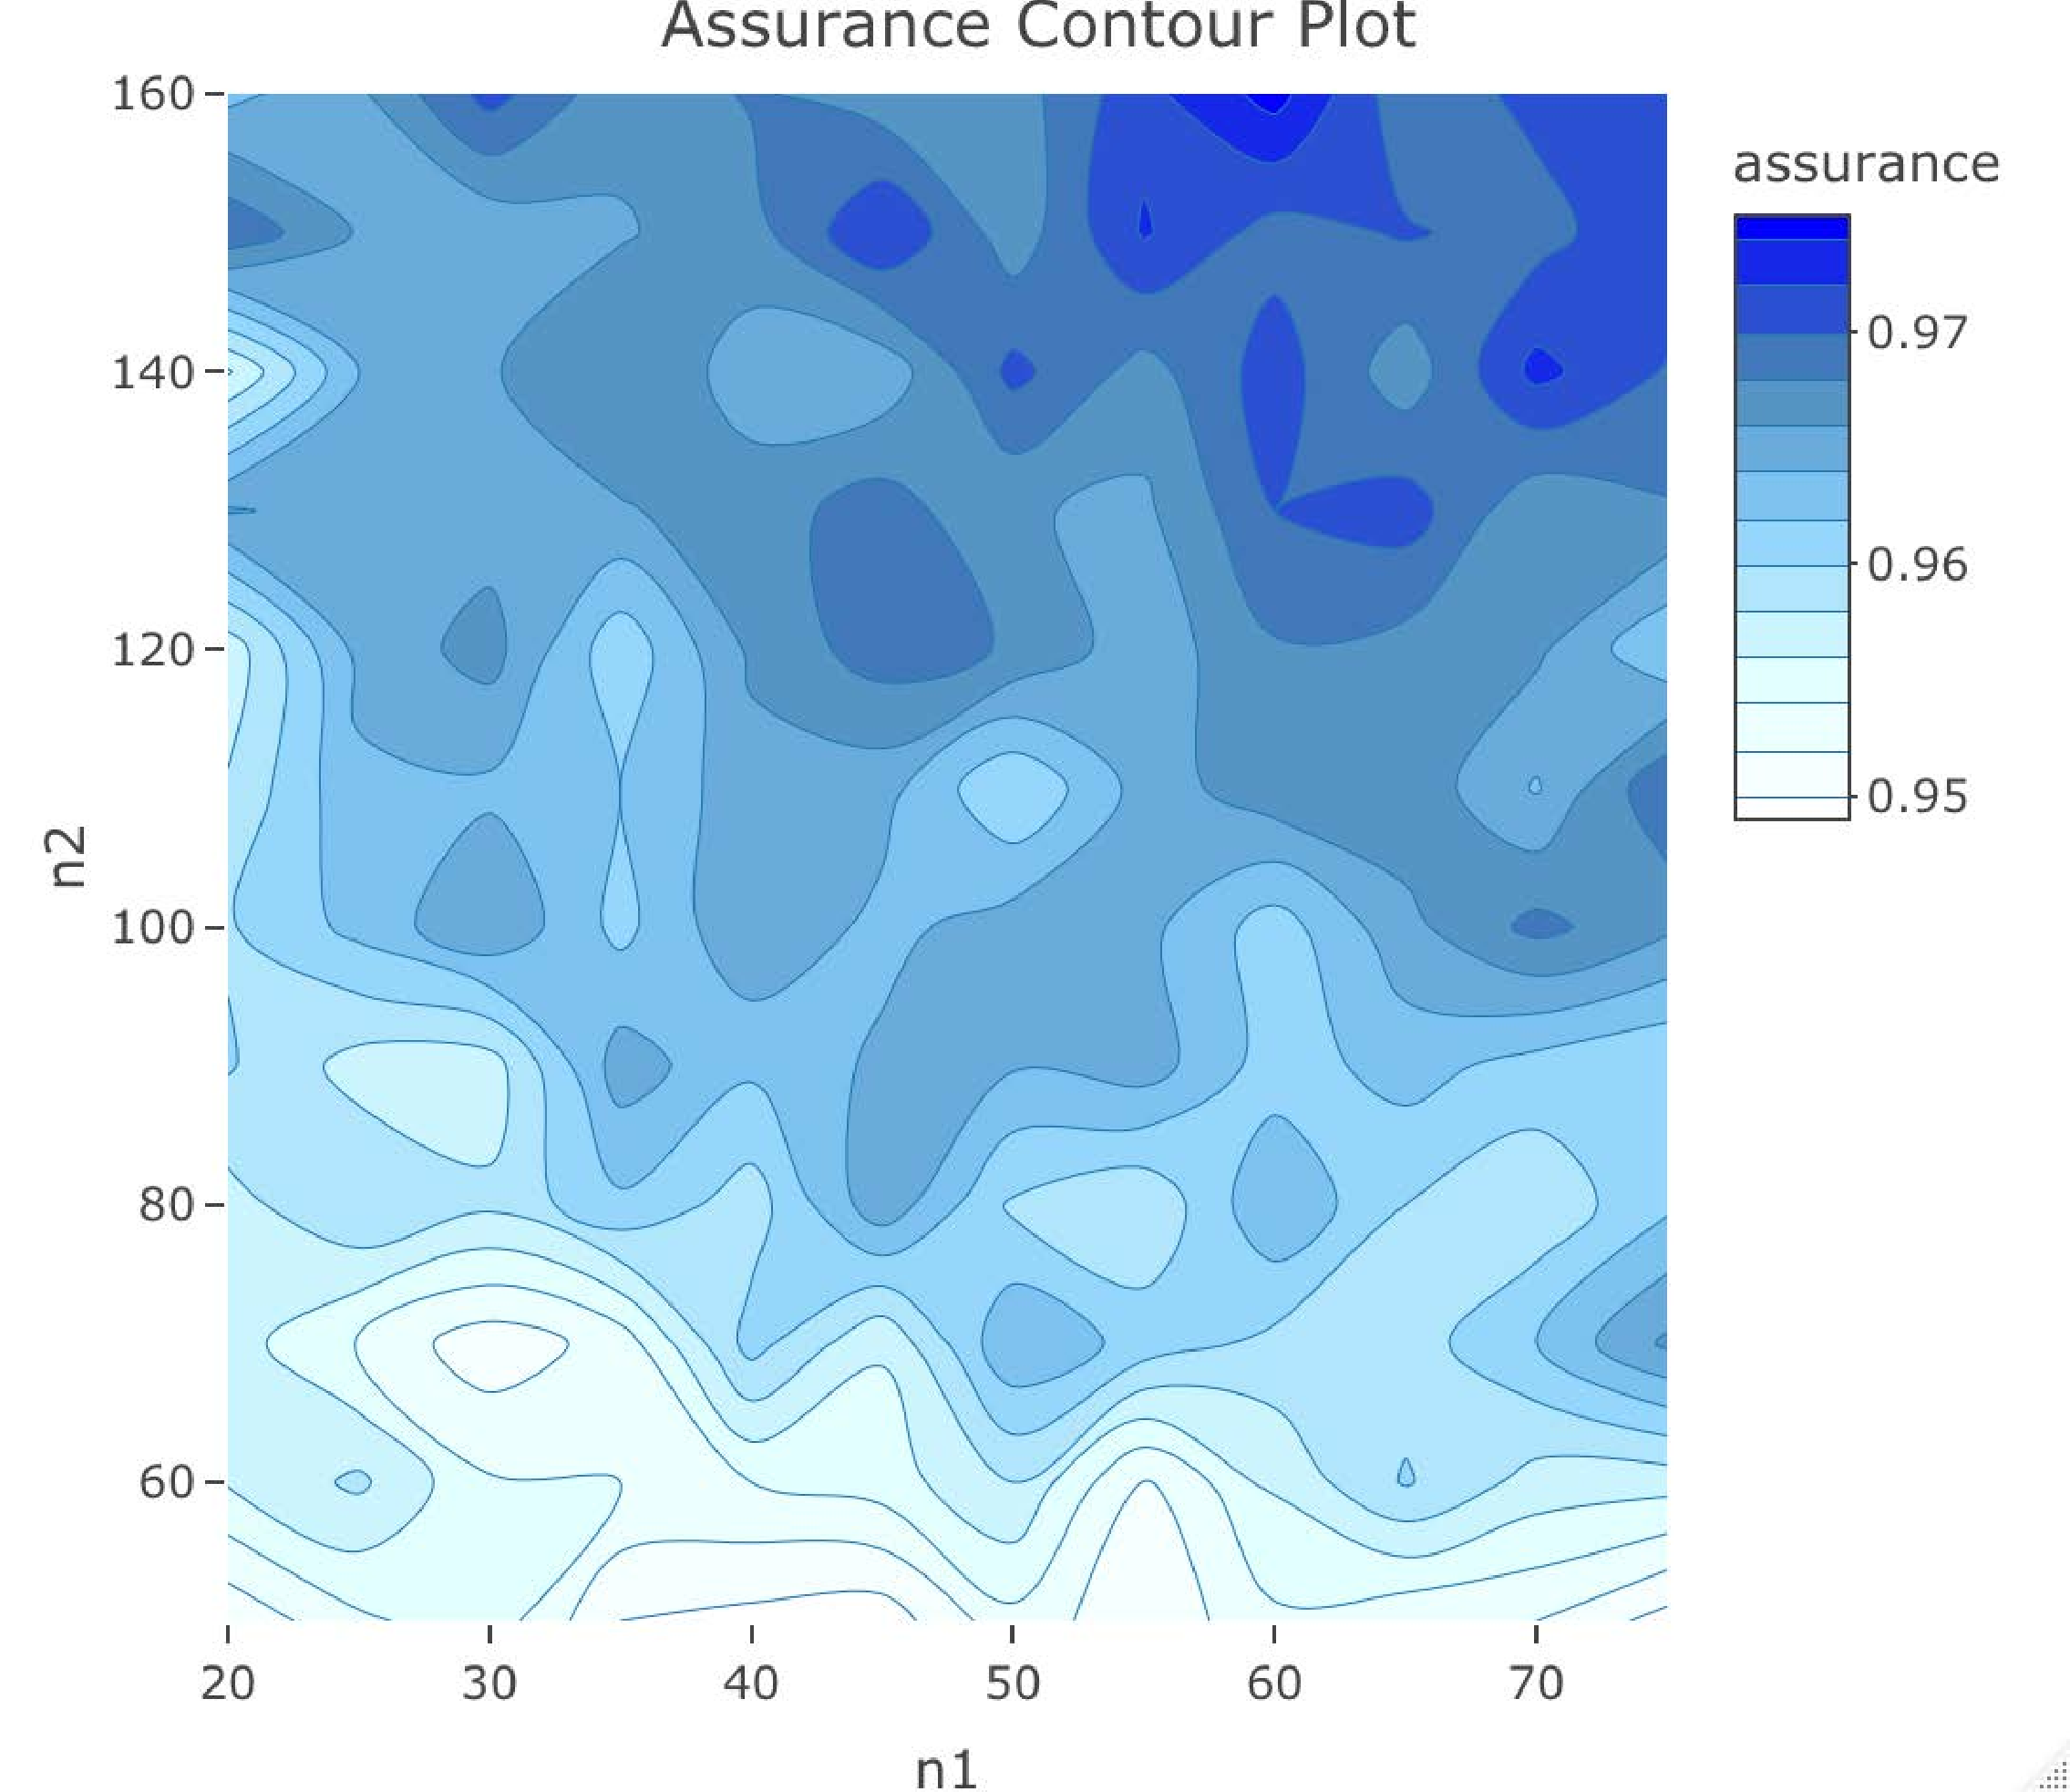
\includegraphics[width = 10 cm]{ex5_contourplot.pdf}
\caption{\label{fig:ex5} Contour map of assurance values with
varying sample sizes \code{n1} and \code{n2}.}
\end{figure}


\subsubsection{Example 5: cost-effectiveness application}
We revisit the cost-effectiveness problem discussed in Example 2. 
In addition to providing
a 3-D graphical display of the assurance, 
this example also demonstrates how the   
\code{repeats} parameter is applied. 

Recall from Example 2 that two distinct sets of efficacy and
cost measures are used to compare the cost-effectiveness 
of treatments 1 and 2. The efficacy and costs
are denoted by $\mu_i$ and $\gamma_i$ for 
$i = 1, 2$ treatments. Hence, the parameter we want to
estimate contains four elements tied to the unknown
efficacy and costs of treatments 1 and 2, i.e.
$\beta = (\mu_1, \gamma_1, \mu_2, \gamma_2)^{\top}$. 
It was previously assumed that the treatments contain an equal number of observations,
suggesting that the sample sizes across each of the four explanatory variables are also equal. Using \fct{bayes\_sim\_unbalanced} 
offers the added flexibility of constructing an unbalanced 
study design between treatments 1
and 2.  Since the two treatments each contain two components
to be measured, we use the \code{repeats} parameter to indicate
that we want two sets of sample sizes, \code{c(n1, n2)}, passed in, 
i.e. \code{c(n1, n2, n1, n2)}. It then becomes clear that our
study design consists of $n_1$ observations for the efficacy
and cost of treatment 1, and $n_2$ observations for those
of treatment 2.  Figure~\ref{fig:ex6} displays a contour plot
with a noticeable increasing trend of assurance values across 
larger sets of sample sizes. 

\begin{Schunk}
\begin{Sin}
R> library(bayesassurance)
R> n1 <- c(4, 5, 15, 25, 30, 100, 200)
R> n2 <- c(8, 10, 20, 40, 50, 200, 250)

R> mu_beta_d <- as.matrix(c(5, 6000, 6.5, 7200))
R> mu_beta_a <- as.matrix(rep(0, 4))
R> K = 20000 # threshold unit cost
R> C <- 0
R> u <- as.matrix(c(-K, 1, K, -1))
R> sigsq <- 4.04^2
R> Vbeta_a_inv <- matrix(rep(0, 16), nrow = 4, ncol = 4)
R> Vbeta_d <- (1 / sigsq) * matrix(c(4, 0, 3, 0, 0, 10^7, 0, 0, 
3, 0, 4, 0, 0, 0, 0, 10^7),nrow = 4, ncol = 4)

R> assur_out <- bayes_sim_unbalanced(n1 = n1, n2 = n2, repeats = 2, 
		u = as.matrix(c(-K, 1, K, -1)), C = 0, Xn = NULL, 
		Vbeta_d = Vbeta_d, Vbeta_a_inv = Vbeta_a_inv,
		Vn = NULL, sigsq = 4.04^2, 
		mu_beta_d = as.matrix(c(5, 6000, 6.5, 7200)), 
		mu_beta_a = as.matrix(rep(0, 4)), 
		alt = "greater", alpha = 0.05, mc_iter = 5000,  
		surface_plot = TRUE)
		
R> assur_out$assurance_table
R> assur_out$contourplot
\end{Sin}
\begin{Sout}
   n1  n2 Assurance
1   4   8    0.1614
2   5  10    0.1724
3  15  20    0.3162
4  25  40    0.3942
5  30  50    0.4440
6 100 200    0.6184
7 200 250    0.7022
\end{Sout}
\end{Schunk}

\begin{figure}[t!]
\centering
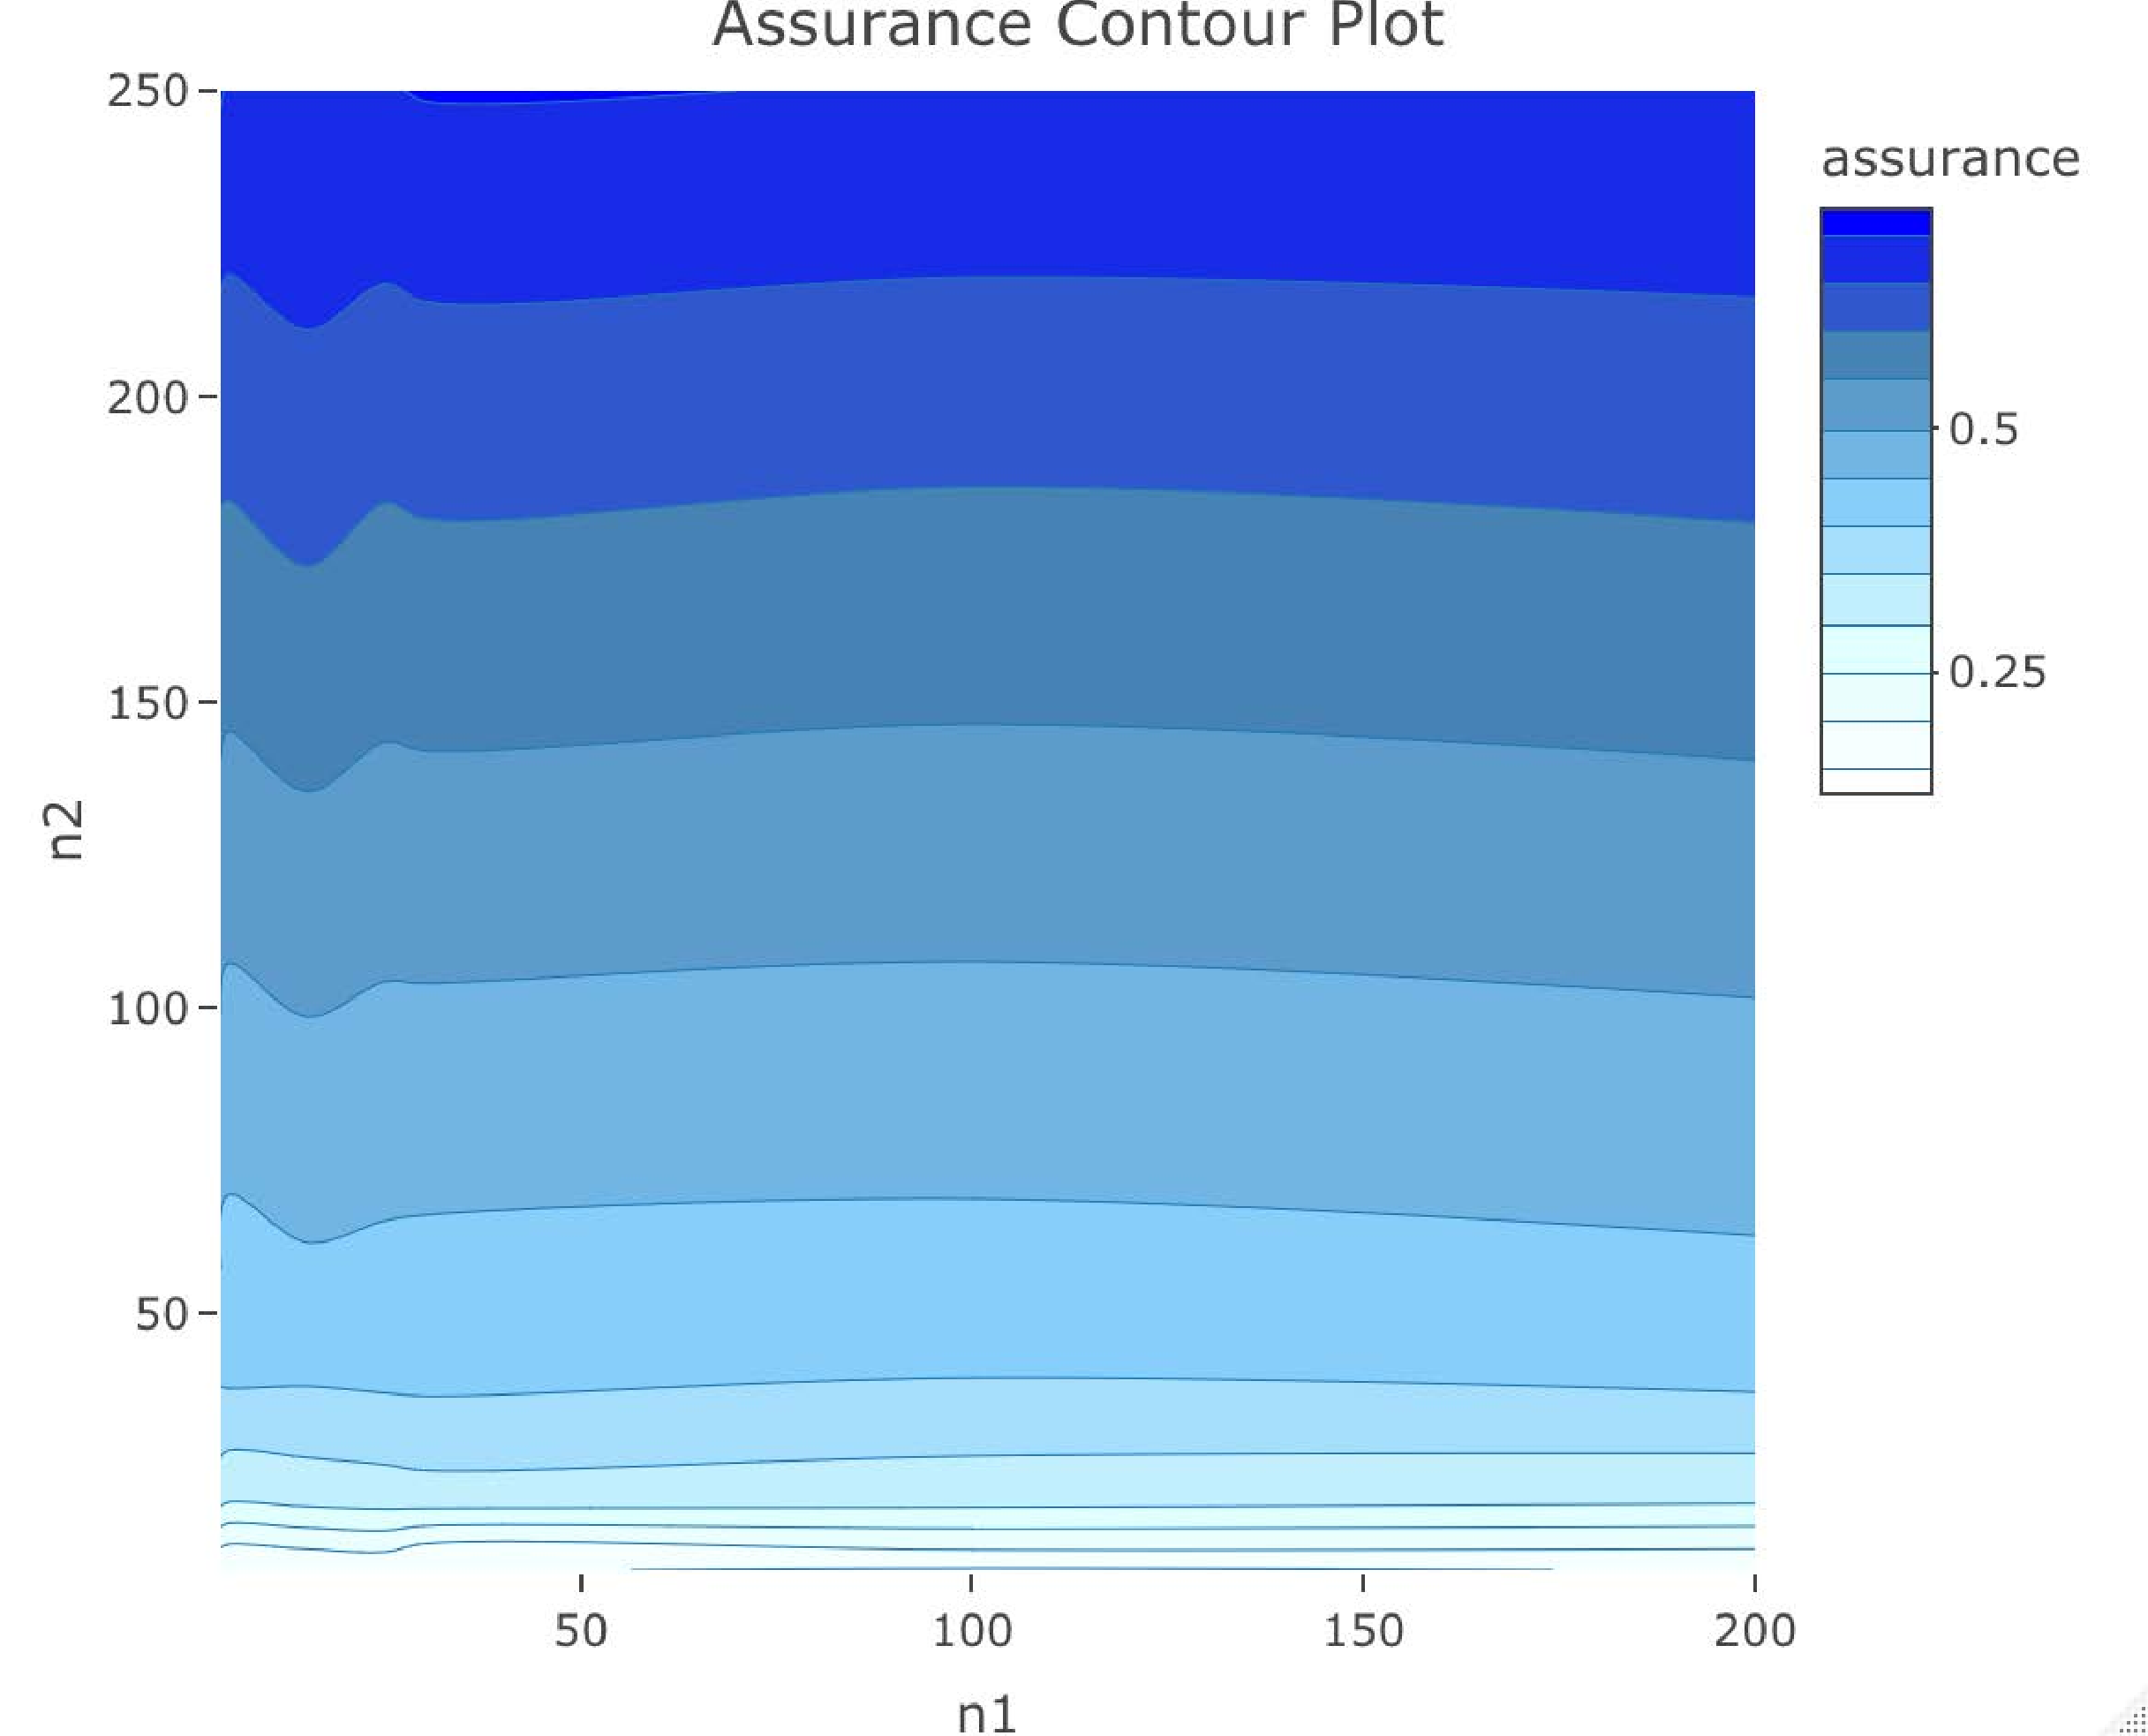
\includegraphics[width = 10 cm]{ex6_contourplot.pdf}
\caption{\label{fig:ex6} Contour map of assurance values in
cost-effectiveness application.}
\end{figure}



\section{Bayesian assurance using other conditions}
\label{sec:othermethods}

The \pkg{bayesassurance} \proglang{R} package contains several other 
assurance functions characterized by analysis stage 
objectives that are dependent on fixed 
precision levels \citep{cj} and posterior credible intervals 
\citep{pham}. These functions are denoted respectively as 
\fct{bayes\_adcock} and \fct{bayes\_sim\_betabin}.
The package also includes a \fct{bayes\_goal\_func} function 
framed under a utility-based setting \citep[see, e.g.,][]{raiffa, berger, lindley, parm, parmigiani, inoue}
that determines sample size in relation to the rate of correct 
classification \citep{inoue}. 
Since the simulation-based assurance functions all follow a similar format,
for the sake of brevity, we will not include detailed descriptions
of them in this article. Vignettes outlining detailed 
descriptions and walkthrough
tutorials can be found on our Github 
page (\href{https://github.com/jpan928/bayesassurance_rpackage}{https://github.com/jpan928/bayesassurance\_rpackage}), which contains examples that users can easily follow along 
and reproduce on their own machines. 




\section[Visualization features and useful tools]{Visualization Features and Useful Tools} \label{sec:tools}

\subsection{Overlapping power and assurance curves}

To facilitate an understanding of the relationship held between
Bayesian and frequentist power analysis, the \fct{pwr\_curves} function 
produces a single plot displaying both power and assurance points. 
%overlayed on top of one another.  
Recall that the primary difference held between
\fct{pwr\_freq} and \fct{assurance\_nd\_na}
is the need to specify additional precision parameters, 
$n_a$ and $n_d$, in \fct{assurance\_nd\_na}. 
Knowing that power and sample size analysis in the frequentist setting
is essentially a special case of the Bayesian assurance 
with precision parameters tailored to weak analysis priors
and strong design priors, the \fct{pwr\_curves} function
serves as a visualization tool in seeing how varying precision levels
affect assurance values and how these assurance values 
compare to those we would expect under classical/frequentist
power analysis (strong design priors, weak analysis priors). 
%of strictly weak analysis and strong design priors, i.e. power values.

The \fct{pwr\_curves} function takes the combined set of
parameters presented in \fct{pwr\_freq} and \fct{assurance\_nd\_na},
which includes \code{n, n\_a, n\_d, theta\_0, theta\_1, sigsq,} and
\code{alpha}. For further customization, users have the option to
include a third set of points in their plot along with the power and
assurance curves. These additional points would correspond to the
simulated assurance results obtained using \fct{bayes\_sim}.
Optional parameters to implement this include 
\begin{enumerate}
	\item{\code{bayes\_sim}: logical that indicates whether the 
	user wishes to include simulated assurance results obtained
	from \fct{bayes\_sim}.  Default setting is
	 \code{FALSE}.}
	\item{\code{mc\_iter}: specifies the number of MC samples 
	to evaluate given \code{bayes\_sim = TRUE}.}
\end{enumerate}
The following code segment runs the \fct{pwr\_curves} function 
using a weak analysis stage prior (\code{n\_a} is
set to be small) and a strong design stage prior (\code{n\_d} is
set to be large). Implementing this produces a plot where the
assurance points lay perfectly on top of the power curve as
shown in Figure~\ref{fig:pwr_curve_ex1}. The simulated assurance
points obtained from \fct{bayes\_sim} are also plotted as we set
\code{bayes\_sim = TRUE}. These points are highlighted in blue, which 
lie very close in proximity to those of the exact
assurance points highlighted in red. 
We can also view individual tables of the three sets of 
points by directly calling them from the saved outputs, e.g.
\code{out\$power\_table} shows the individual frequentist
power values for each sample size. The output we provide
shows the first ten rows. 

\begin{figure}[t!]
\centering
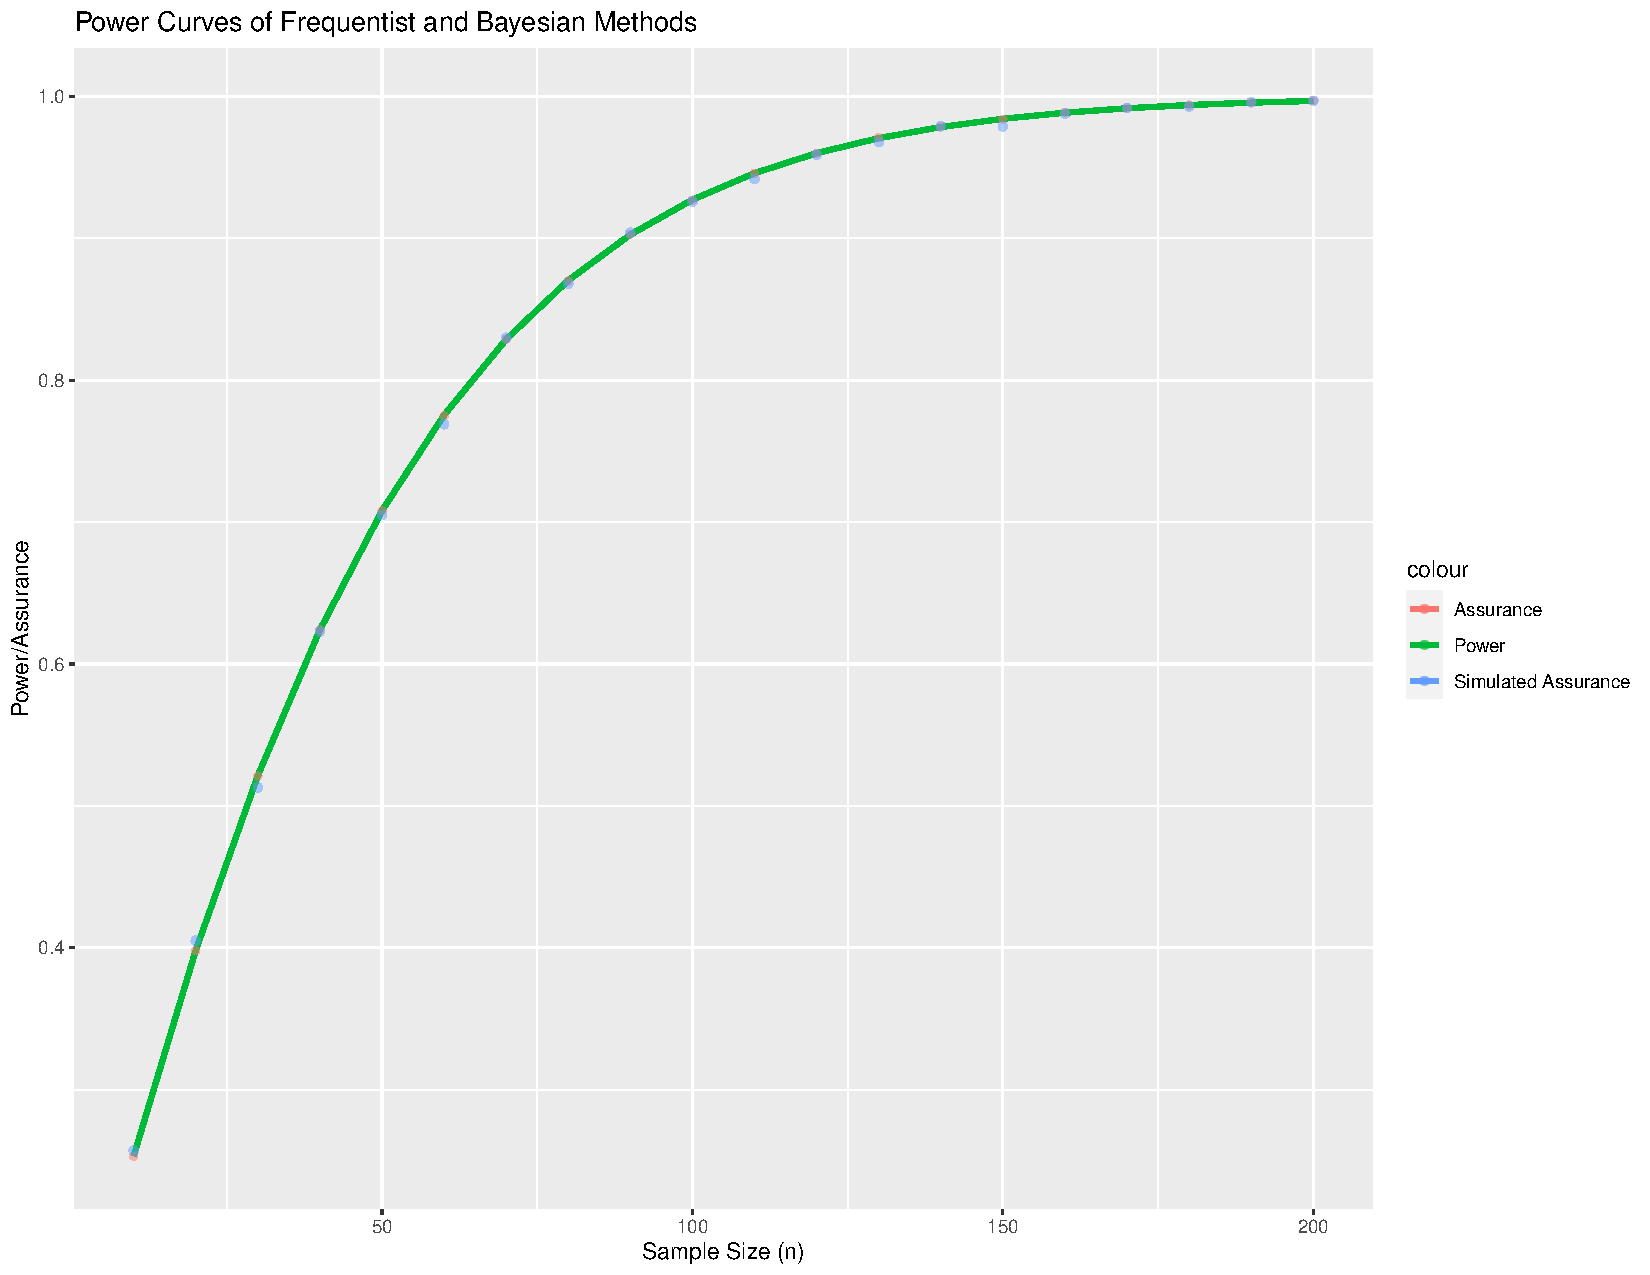
\includegraphics[width = 10 cm]{pwr_curve_ex1.pdf}
\caption{\label{fig:pwr_curve_ex1} Power curve with exact and simulated
assurance points for weak analysis prior and strong design prior.}
\end{figure}

\begin{Schunk}
\begin{Sin}
R> library(bayesassurance)

R> out <- pwr_curve(n = seq(10, 200, 10), n_a = 1e-8, n_d = 1e+8, 
        sigsq = 0.104, theta_0 = 0.15,theta_1 = 0.25, alt = "greater", alpha = 0.05, 
        bayes_sim = TRUE, mc_iter = 5000)

R> head(out$power_table)
R> head(out$assurance_table)
R> out$plot

\end{Sin}
\begin{Sout}
     n     Power
1   10 0.2532578
2   20 0.3981637
3   30 0.5213579
4   40 0.6241155
5   50 0.7080824
6   60 0.7754956

     n Assurance
1   10 0.2532578
2   20 0.3981637
3   30 0.5213579
4   40 0.6241155
5   50 0.7080824
6   60 0.7754956
\end{Sout}
\end{Schunk}


The next code segment considers the scenario in which both analysis
and design stage priors are weak (\code{n\_a} 
and \code{n\_d} are set to be small). This special case
shows how the assurance behaves when vague
priors are assigned. 
Substituting 0 in for both $n_a$ and $n_d$ in
Equation~\eqref{eq:assurance} results in a constant
assurance of $\Phi(0) = 0.5$ regardless of the sample size
and critical difference.  Figure~\ref{fig:pwr_curve_ex2} illustrates
these results, where we have the regular power curve and
the flat set of assurance points at 0.5 for both exact and simulated
cases. 
%Note that some of these points appear purple due to the overlaps that occur between the exact and simulated assurance values. 

\begin{figure}[t!]
\centering
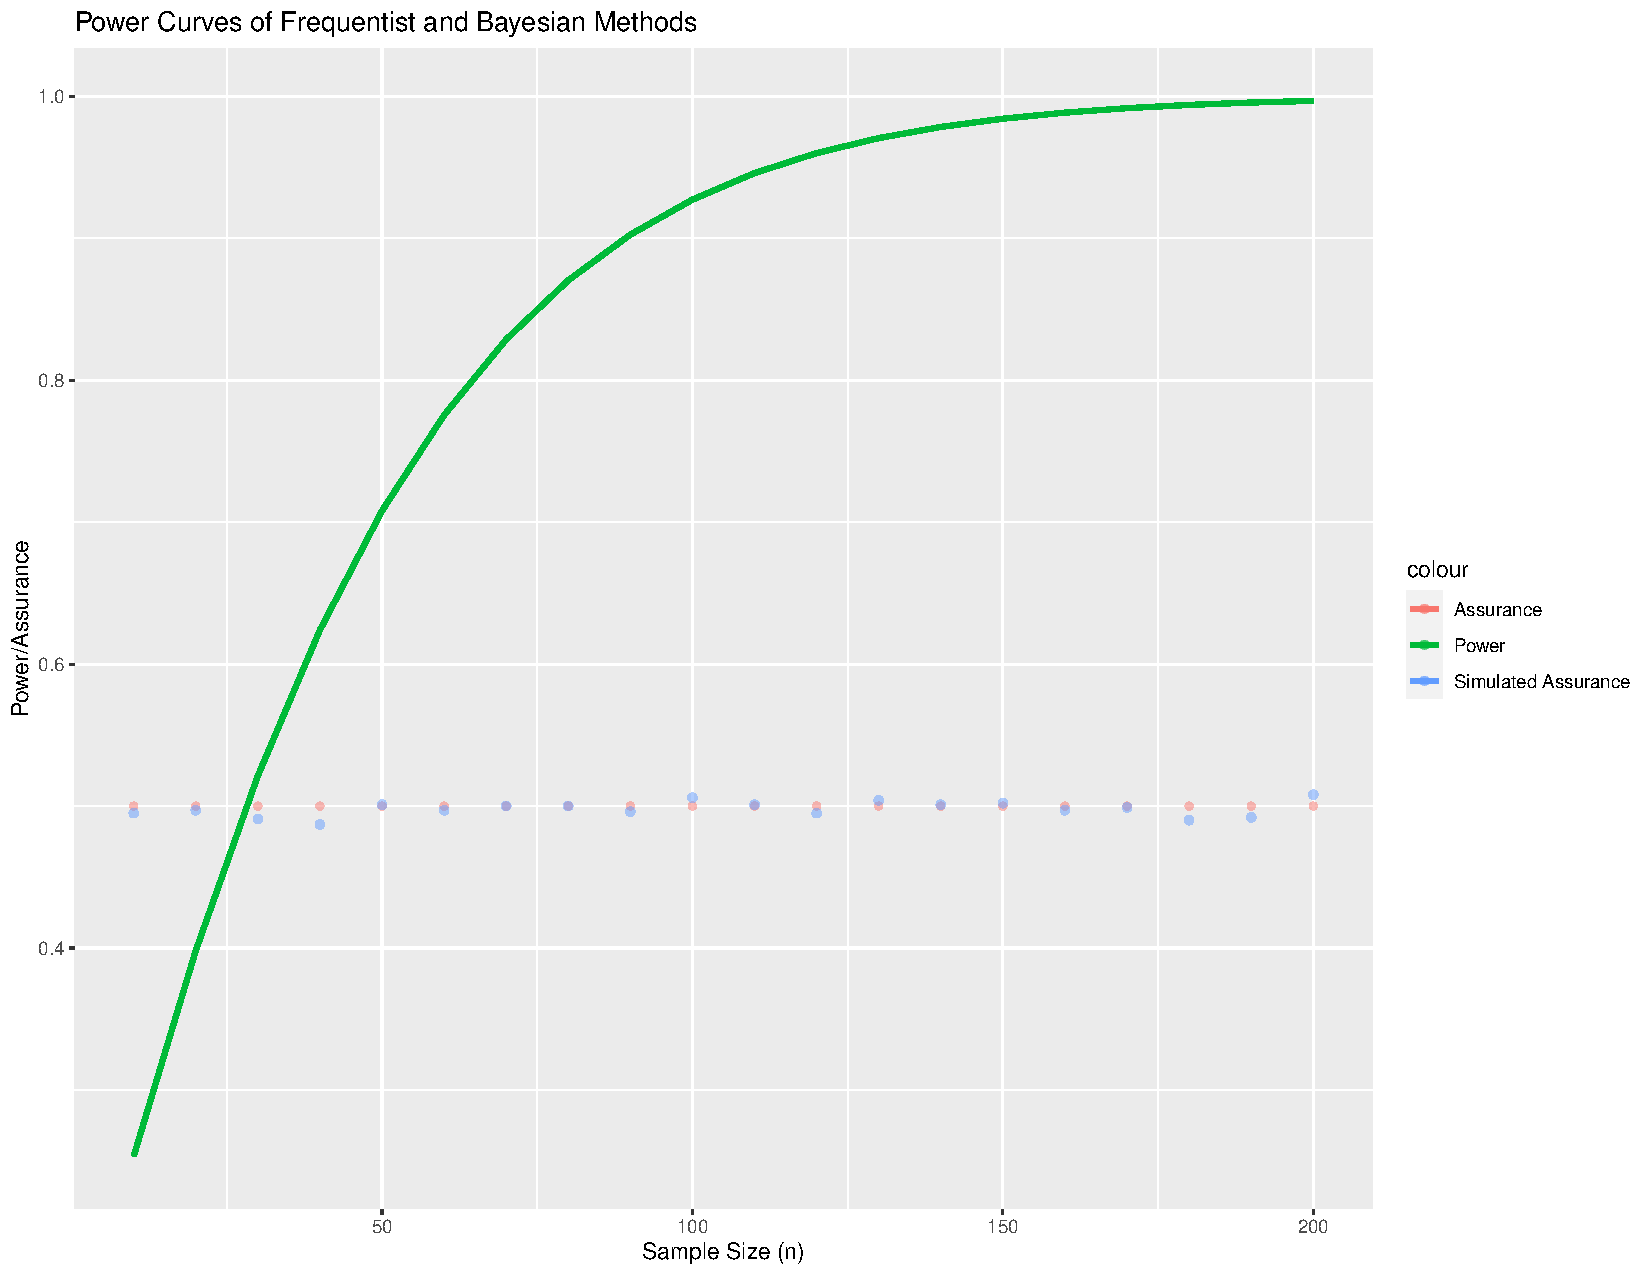
\includegraphics[width = 8 cm]{pwr_curve_ex2.pdf}
\caption{\label{fig:pwr_curve_ex2} Power curve with exact and simulated
assurance points for weak analysis and design priors.}
\end{figure}

\begin{Schunk}
\begin{Sin}
R> library(bayesassurance)

R> pwr_curve(n = seq(10, 200, 10), n_a = 1e-8, n_d = 1e-8, 
sigsq = 0.104, theta_0 = 0.15,theta_1 = 0.25, alt = "greater", alpha = 0.05, 
bayes_sim = TRUE, mc_iter = 5000)

\end{Sin}
\end{Schunk}





\subsection{Design matrix generators}\label{design_matrix_generators}
In the last few sections, we go over design matrix generators
that are used inside functions within
the \pkg{bayesassurance} package when the \code{Xn}
parameter is set to \code{NULL}.
We include these functions in case users wish to see 
how design matrices are constructed under this particular
setting. 

\subsubsection{Standard design matrix generator}\label{subsubsec:standard_designmatrix}
The standard design matrix generator, \fct{gen\_Xn}, 
is relevant to a majority of the simulation-based assurance
functions discussed throughout the paper. 
%It is first mentioned in Section~\ref{sec:simform} that the assurance function under known variance,\fct{bayes\_sim}, 
It should be noted that all simulation-based functions
available in this package
do not require users to specify their own
design matrix $X_n$. Users have the option of leaving 
\code{Xn = NULL}, which prompts the function to construct a 
default design matrix using \fct{gen\_Xn} that complies
with the general linear model $y_n = X_n\beta +
\epsilon$, $\epsilon \sim N(0, \sigma^2V_n)$. The function
runs in the background while 
\fct{bayes\_sim} is used.

When called directly, 
the \fct{gen\_Xn} function takes in a single parameter, 
\code{n}, which can either be a scalar or vector. 
The length of \code{n} corresponds
to the number of groups being assessed in the study design
as well as the column dimension of the design matrix,
denoted as \code{p}. Therefore, in general, the resulting 
design matrix is of dimension $n \times p$. 
If a scalar value is specified for \code{n}, 
the resulting design matrix carries a dimension
of $n \times 1$. 

In the following example, we pass in a vector
of length $p = 4$, which outputs a design matrix of 
column dimension 4. Each column is comprised 
of ones vectors with lengths 
that align with the sample sizes passed in for
\code{n}. The row dimension is therefore the sum 
of all the entries in \code{n}. 
In this case, since the values 1, 3, 5, and 8 are
being passed in to \code{n}, the design matrix
to be constructed carries a row dimension of 
$1 + 3 + 5 + 8 = 17$ and a column dimension of 4. 

\begin{Schunk}
\begin{Sin}
R> n <- c(1,3,5,8)
R> gen_Xn(n = n)
\end{Sin}
\begin{Sout}
      [,1] [,2] [,3] [,4]
 [1,]    1    0    0    0
 [2,]    0    1    0    0
 [3,]    0    1    0    0
 [4,]    0    1    0    0
 [5,]    0    0    1    0
 [6,]    0    0    1    0
 [7,]    0    0    1    0
 [8,]    0    0    1    0
 [9,]    0    0    1    0
[10,]    0    0    0    1
[11,]    0    0    0    1
[12,]    0    0    0    1
[13,]    0    0    0    1
[14,]    0    0    0    1
[15,]    0    0    0    1
[16,]    0    0    0    1
[17,]    0    0    0    1
\end{Sout}
\end{Schunk}

The \fct{bayes\_sim} function and its related family of 
functions generate design matrices using \fct{gen\_Xn} 
in the following way. 
Each unique value contained in \code{n} that is
passed into \fct{bayes\_sim} corresponds to a distinct
study design and thus requires a distinct
design matrix. The \fct{gen\_Xn} function interprets each 
$i^{th}$ component of \code{n} as a separate balanced study 
design comprised of $n_i$ participants within each of the $p$
groups, where \code{p} is a parameter specified
in \fct{bayes\_sim}. For example, if we let 
\code{Xn = NULL} and pass in 
\code{n <- 2}, \code{p <- 4} for \fct{bayes\_sim},  
\fct{gen\_Xn} will process the vector
\code{n <- c(2, 2, 2, 2)} in the background. Hence, we'd obtain an 
$8 \times 4$ matrix of the form
\[
X_n = 
\begin{bmatrix}
1 & 0 & 0 & 0 \\
1 & 0 & 0 & 0 \\
0 & 1 & 0 & 0 \\
0 & 1 & 0 & 0 \\
0 & 0 & 1 & 0 \\
0 & 0 & 1 & 0 \\
0 & 0 & 0 & 1 \\
0 & 0 & 0 & 1 \\
\end{bmatrix}.
\]



\subsubsection{Design matrix generator in longitudinal setting}\label{subsubsec:long_designmatrix}
Example 3 demonstrates how the 
linear model is extended to incorporate time-based 
covariates within the context of a longitudinal setting. For this
special case, a separate function is used to generate
design matrices that are appropriate for this setting. 
The \fct{genXn\_longitudinal} constructs
its design matrices differently than \fct{gen\_Xn} 
and therefore requires a different set of parameter specifications.
When the \code{longitudinal} parameter is
set to \code{TRUE} in \fct{bayes\_sim}, 
the user is required to specify the following set
of parameters, which are directly passed into 
\fct{genXn\_longitudinal}: 

\begin{enumerate}
\item{\code{ids}: vector of unique subject ids, usually of length 2
for study design purposes}
\item{\code{from}: start time of repeated measures for
each subject}
\item{\code{to}: end time of repeated measures for
each subject}
\item{\code{num\_repeated\_measures}: desired length of the repeated measures sequence. Should be a non-negative number, will be rounded up if fractional.}
\item{\code{poly\_degree}:  degree of polynomial in longitudinal model, set to 1 by default.}
\end{enumerate}

Referring back to the model that was constructed for the 
case involving two subjects,  we observe in 
Equation~\eqref{eq:long_model} that the
design matrix contains vectors of ones within the first half
of its column dimension and lists the timepoints 
for each subject in the second half. Constructing this
design matrix requires several components. The user needs to
specify subject IDs that are capable of uniquely
identifying each individual in the study.  
Next, the user needs to specify the start and end time 
as well as the number of repeated measures reported 
for each subject. The number of repeated measures 
denotes the number of evenly-spaced timepoints that 
take place in between the start and end time. 
Since we are assuming a balanced longitudinal 
study design, each subject
considers the same set of timepoints. Finally, if the user
wishes to consider time covariates of higher degrees, such as 
a quadratic or cubic function, this can be altered using 
the \code{poly\_degree} parameter, which takes on
a default assignment of 1. 

In the following code, we pass in a vector of 
subject IDs and specify the start and end
timepoints along with the desired length of the sequence.
The resulting design matrix contains vectors of
ones with lengths that correspond to the number of repeated
measures for each unique subject.

\begin{Schunk}
\begin{Sin}
 R> ids <- c(1,2,3,4)
 R> gen_Xn_longitudinal(ids, from = 1, to = 10, num_repeated_measures = 4)
\end{Sin}
\begin{Sout}
      [,1] [,2] [,3] [,4] [,5] [,6] [,7] [,8]
 [1,]    1    0    0    0    1    0    0    0
 [2,]    1    0    0    0    4    0    0    0
 [3,]    1    0    0    0    7    0    0    0
 [4,]    1    0    0    0   10    0    0    0
 [5,]    0    1    0    0    0    1    0    0
 [6,]    0    1    0    0    0    4    0    0
 [7,]    0    1    0    0    0    7    0    0
 [8,]    0    1    0    0    0   10    0    0
 [9,]    0    0    1    0    0    0    1    0
[10,]    0    0    1    0    0    0    4    0
[11,]    0    0    1    0    0    0    7    0
[12,]    0    0    1    0    0    0   10    0
[13,]    0    0    0    1    0    0    0    1
[14,]    0    0    0    1    0    0    0    4
[15,]    0    0    0    1    0    0    0    7
[16,]    0    0    0    1    0    0    0   10
\end{Sout}
\end{Schunk}

The next code block modifies the previous example 
to incorporate a quadratic term. Notice there are 
four additional columns being aggregated to the design matrix. 
These four columns are obtained from squaring
the four columns of the linear term. 
\begin{Schunk}
\begin{Sin}
 R> ids <- c(1,2,3,4)
 R> gen_Xn_longitudinal(ids, from = 1, to = 10, num_repeated_measures = 4, 
 poly_degree = 2)
\end{Sin}
\begin{Sout}
      1 2 3 4  1  2  3  4   1   2   3   4
 [1,] 1 0 0 0  1  0  0  0   1   0   0   0
 [2,] 1 0 0 0  4  0  0  0  16   0   0   0
 [3,] 1 0 0 0  7  0  0  0  49   0   0   0
 [4,] 1 0 0 0 10  0  0  0 100   0   0   0
 [5,] 0 1 0 0  0  1  0  0   0   1   0   0
 [6,] 0 1 0 0  0  4  0  0   0  16   0   0
 [7,] 0 1 0 0  0  7  0  0   0  49   0   0
 [8,] 0 1 0 0  0 10  0  0   0 100   0   0
 [9,] 0 0 1 0  0  0  1  0   0   0   1   0
[10,] 0 0 1 0  0  0  4  0   0   0  16   0
[11,] 0 0 1 0  0  0  7  0   0   0  49   0
[12,] 0 0 1 0  0  0 10  0   0   0 100   0
[13,] 0 0 0 1  0  0  0  1   0   0   0   1
[14,] 0 0 0 1  0  0  0  4   0   0   0  16
[15,] 0 0 0 1  0  0  0  7   0   0   0  49
[16,] 0 0 0 1  0  0  0 10   0   0   0 100
\end{Sout}
\end{Schunk}


\section{Discussion}
This article introduced \pkg{bayesassurance},
a new \proglang{R} package for computing Bayesian assurance under various conditions using a two-stage framework.  The goal of this package is to provide a convenient and user-friendly interface to statisticians and data scientists who seek sample size calculations using the assurance function in Bayesian data analysis. We have attempted to provide an organized, well-documented open-source code that can be used to address a wide range of study design problems, such as in the case of clinical trials, and demonstrate the feasibility
of applying Bayesian methods to such problems.





\hypertarget{refs}{}

\bibliography{jpan.bib}

\address{%
Jane Pan\\
University of California, Los Angeles\\%
650 Charles E Young Dr S, Los Angeles, CA 90095\\ USA\\
%
%
%
\href{mailto:jpan1@ucla.edu}{\nolinkurl{jpan1@ucla.edu}}%
}

\address{%
Sudipto Banerjee\\
University of California, Los Angeles\\%
650 Charles E Young Dr S, Los Angeles, CA 90095\\ USA\\
%
%
%
\href{mailto:sudipto@ucla.edu}{\nolinkurl{sudipto@ucla.edu}}%
}

\end{article}


\end{document}
